\documentclass{beamer}



\mode<presentation> %
{
  % \usetheme{Warsaw}
  % or ...
%\usetheme{Madrid}%https://www.overleaf.com/learn/latex/Beamer#Reference_guide
  % \usetheme{AnnArbor}
  % \usetheme{PaloAlto}
%   \usetheme{Darmstadt}
  \usetheme{EastLansing}
%   \usecolortheme{rose}


%   \usecolortheme{wolverine}
  \setbeamercovered{transparent}
  \setbeamerfont{caption}{size=\scriptsize}
  % or whatever (possibly just delete it)
}
% \usepackage{appendixnumberbeamer}

\usepackage{array}
\usepackage{tabularx} 
\usepackage{multirow}
%\usepackage{longtable}
%\usepackage{subfigure}not found
%\usepackage{lipsum}
%\usepackage[demo]{graphicx}
\usepackage{graphicx}
\usepackage{graphicx,subcaption}
\usepackage{caption}
\usepackage{subcaption}
\usepackage{xcolor}
% \usepackage{ulem}
\usepackage{soul}
%\usepackage{grffile}
\usepackage{hyperref}

\hypersetup{
    colorlinks=true,
    linkcolor=blue,
    filecolor=magenta,      
    urlcolor=green,
    pdftitle={Overleaf Example},
    pdfpagemode=FullScreen,
    }


\usepackage[english]{babel}
% or whatever

\usepackage[latin1]{inputenc}
% or whatever

\usepackage{times}
\usepackage[T1]{fontenc}
% Or whatever. Note that the encoding and the font should match. If T1
% does not look nice, try deleting the line with the fontenc.
\usepackage{hyperref}
\beamertemplatenavigationsymbolsempty

\title[Rounds 5-6 LD sensors] % (optional, use only with long paper titles)
{IV+CV results of Rounds 5-6 LD sensors}
%\subtitle
%{Include Only If Paper Has a Subtitle}
\author[Huiling Hua, Marta Krawczyk] % (optional, for multiple authors)
% {Huiling Hua }
{ Pedro Almeida\and Nicholas Adams\and \textbf{Huiling Hua} \and Lucie Linssen\and Filip Moortgat\and Thorben Quast\and Kourosh Sarbandi\and Eva Sicking\and
Chaochen Yuan\and Philipp Zehetner\and \textbf{Marta Krawczyk} }
% \titlegraphic{
% 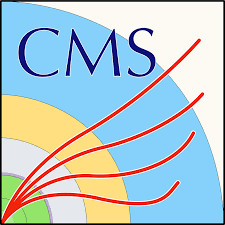
\includegraphics[width=1.0cm]{plots/CMS_Logo.png}
% % \includegraphics[width=1.0cm]{plots}
% }
\logo{
  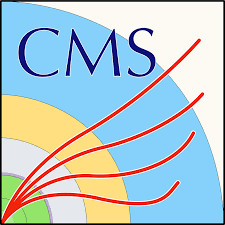
\includegraphics[width=0.7cm]{plots/CMS_Logo.png}
  
\includegraphics[width=0.7cm]{plots/CERN_logo.png}
}

%\author{Huiling Hua}
%\institute{IHEP}
% \institute[IHEP] % (optional)
% {
%   \inst{1}%
%     IHEP
% }
\date[28.04.2022] % (optional, should be abbreviation of conference name)
{HGC Si characterisations at CERN}

% - Either use conference name or its abbreviation.
% - Not really informative to the audience, more for people (including
%   yourself) who are reading the slides online
\subject{Physics Analysis}
% This is only inserted into the PDF information catalog. Can be left
% out. 

% If you have a file called "university-logo-filename.xxx", where xxx
% is a graphic format that can be processed by latex or pdflatex,
% resp., then you can add a logo as follows:
% \pgfdeclareimage[height=0.4.1cm]{university-logo}{university-logo-filename}
% \logo{\pgfuseimage{university-logo}}

% Delete this, if you do not want the table of contents to pop up at
% the beginning of each subsection:
% \AtBeginSubsection[]
% {
  % \begin{frame}<beamer>{Outline}
    % \tableofcontents[currentsection,currentsubsection]
  % \end{frame}
% }
\AtBeginSection[]
{
  \begin{frame}<beamer>{Outline}
    \tableofcontents[currentsection]
    % \addtocounter{framenumber}{-1}
  \end{frame}
}

\begin{document}

\begin{frame}
  \titlepage
\end{frame}

% \begin{frame}{Outline}
%   \tableofcontents
  % You might wish to add the option [pausesections]
% \end{frame}
\section{Introduction}


\begin{frame}{RINSC irradiation, overview}
  \begin{table}[htbp] %[h]
      \centering
      \footnotesize%Use \footnotesize for a 20% (linear) reduction in font size
      \setlength\tabcolsep{2pt}%Reduce the amount of intercolumn whitespace
      \resizebox{0.8\textwidth}{!}{% 
          \begin{tabular}{|c | c |c|} 
           \hline
              & \href{https://indico.cern.ch/event/1121372/contributions/4715417/attachments/2382784/4071626/2-1-2022_Irradiation_Update_from_Brown.pdf}{Round 5}   & \href{https://indico.cern.ch/event/1121372/contributions/4715417/attachments/2382784/4071626/2-1-2022_Irradiation_Update_from_Brown.pdf}{Round 6}\\

           \hline
           \textbf{Date}   & 19.01.2022 &  26.01.2022 \\
           \hline
           \textbf{Target fluence [neq/cm2]}  &   4.00E+15 & 5.50E+15\\
           \hline
           \href{https://indico.cern.ch/event/1121372/contributions/4715417/attachments/2382784/4071626/2-1-2022_Irradiation_Update_from_Brown.pdf}{\textbf{Annealing time in the reactor at $60^{oC}$}}  &  16.1 min (Front: 48.8 min, Back: 9.2 min) & 115.4 min (Front: 961.5 min, Back: 18.6 min)\\
           \hline
           \textbf{Order} (back to front) &   N4790\_08, N4790\_09, N4790\_21 & N4792\_09, N4790\_08, N4792\_20 \\
           \hline
          \end{tabular}
      }
      \end{table}
      
    \begin{columns}
        \column{.5\textwidth}
        \begin{figure}
          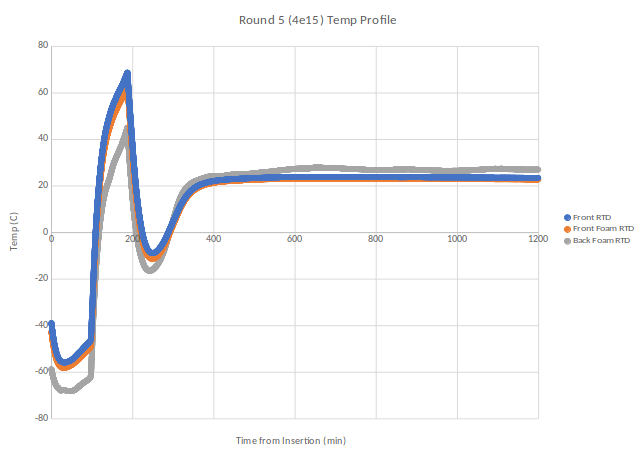
\includegraphics[width=0.9\textwidth]{plots/Round5_temp_profile.png}
          % \caption{Round 5, temperature profile}
        \end{figure}
        \column{.5\textwidth}
        \begin{figure}
          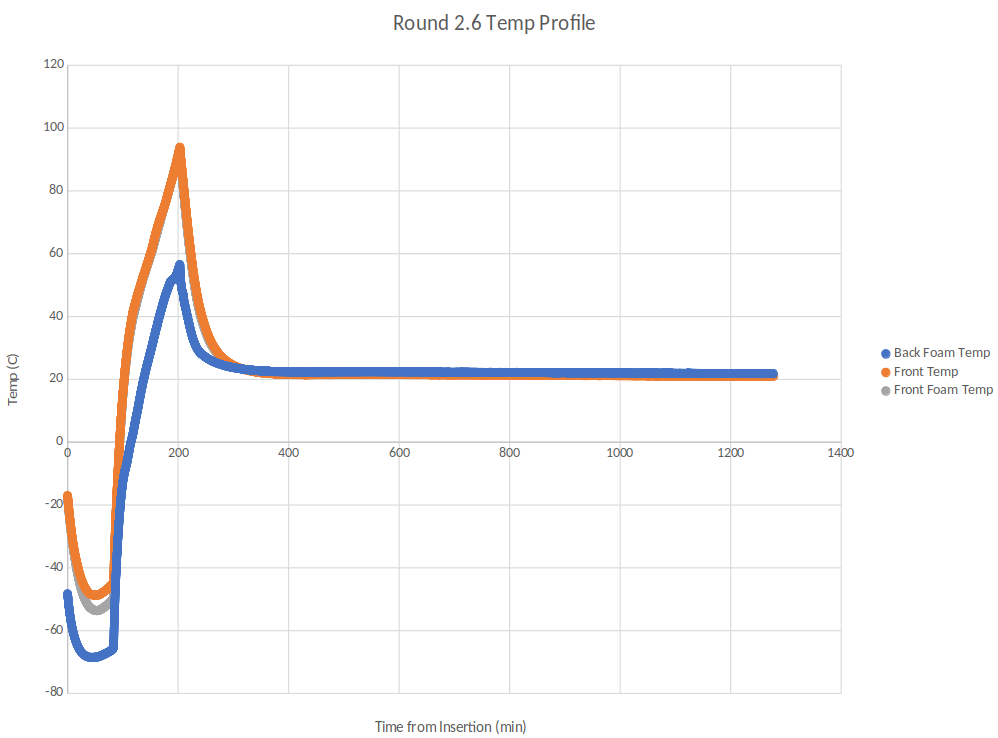
\includegraphics[width=.9\textwidth]{plots/Round6_temp_profile.png}
        \end{figure}
    \end{columns}
  \footnotetext[1]{\href{https://indico.cern.ch/event/1133434/contributions/4755743/attachments/2404163/4112283/RINSC_irradiated_sensors_Rounds1-3\%281\%29.pdf}{More Info about the the profiles.}
  }
\end{frame}



\begin{frame}{Sensor list and annealing step}
%   \begin{figure}
%       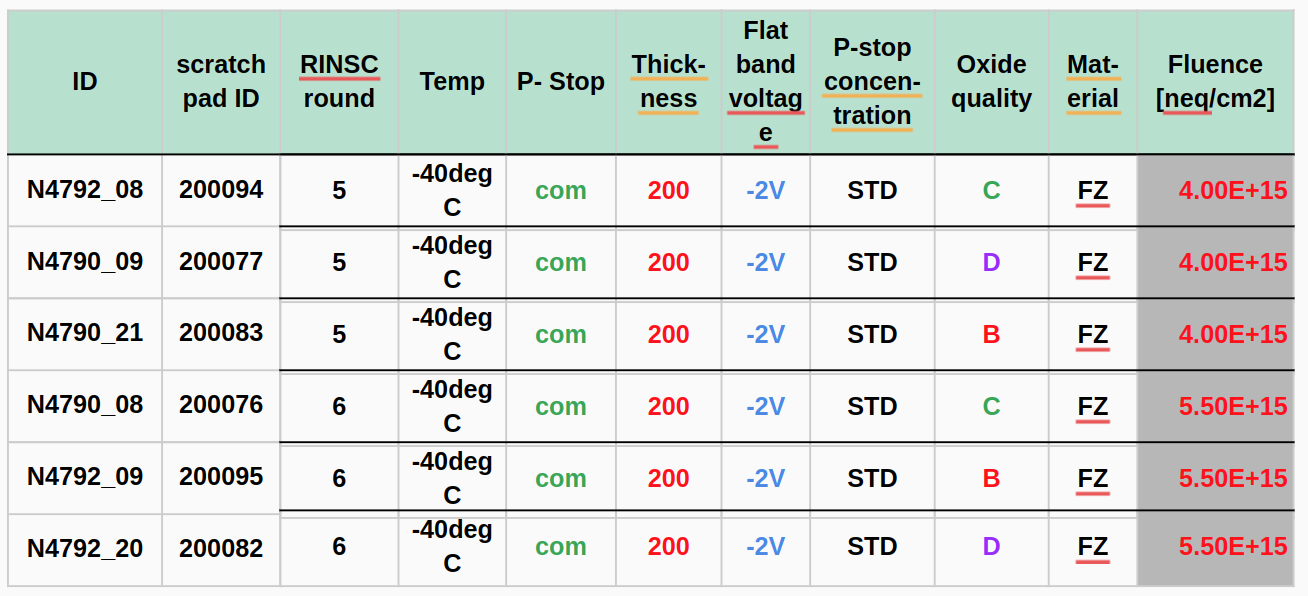
\includegraphics[width=.45\textwidth]{plots/Sensors.png}
%   \end{figure}
    \begin{table}[htbp] %[h]
        \centering
        \footnotesize%Use \footnotesize for a 20% (linear) reduction in font size
        \setlength\tabcolsep{2pt}%Reduce the amount of intercolumn whitespace
        \resizebox{1.0\textwidth}{!}{% 
            \begin{tabular}{|c | c |c|c|} 
             \hline
                sensor &  annealing steps post raditation & IV grading & CV grading \\
             \hline
             N4790\_09  & 27.6min + 31.8min & all passed & inclusive \\ 
             \hline
             N4790\_21 & 10.9min + 11.7min + 11.4min + 9.6min +11.5min + 19.9min+ 11.4min + 17.2min & all passed & inclusive  \\

             \hline
             N4792\_7 & 30.9min +  31.0min  & 0 passed , 30 analysis not run, 60 passed& inclusive \\
             \hline
             \hline
             N4790\_08 & no additional annealing & passed & inclusive \\
             N4792\_09 & no additional annealing & passed & inclusive \\
             N4792\_20 & no additional annealing & analysis not run & inclusive\\
            \hline
            \end{tabular}
        }
        \caption{Annealing steps}
        \end{table}   
  \begin{itemize}
      \small
      \item Sensor N4792\_08 could not be located, instead the sensor N4792\_07 was found in the stack
  \end{itemize}
\end{frame}


\begin{frame}{Measurement Setup: ALPS}
    \begin{figure}
        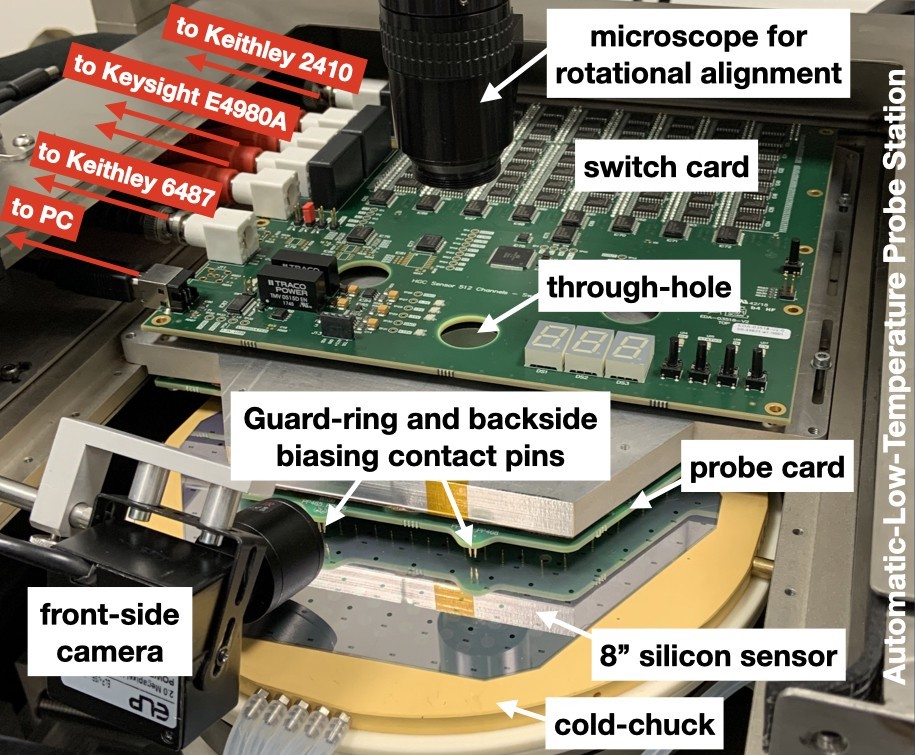
\includegraphics[width=.45\textwidth]{plots/ALPS_setup.png}
    \end{figure}
  
    \begin{itemize}
        % \small
        \scriptsize
        \item Sensors placed directly on chuck (no backside protection)
        \item Temperature: $-40^oC$; humidity: $ 4\% - 8\%$
        \item Voltage provided through the HV pin to the frontside;  voltage up to \alert{-850V}
        \item Annealing at $60^oC$ (chuck), target time of 115 mins
        \item Sensors from Round 5 were annealed to the total time of 115 min at CERN 
        \item Sensors from Round 6 were not further annealed
    \end{itemize}
\end{frame}
  

\section{Annealing effect on IV results}

\subsection{N4790\_21}

\begin{frame}{ Annealing effect on IV (N4790\_21)}
   \begin{columns}
        \column{.5\textwidth}
        \begin{figure}
            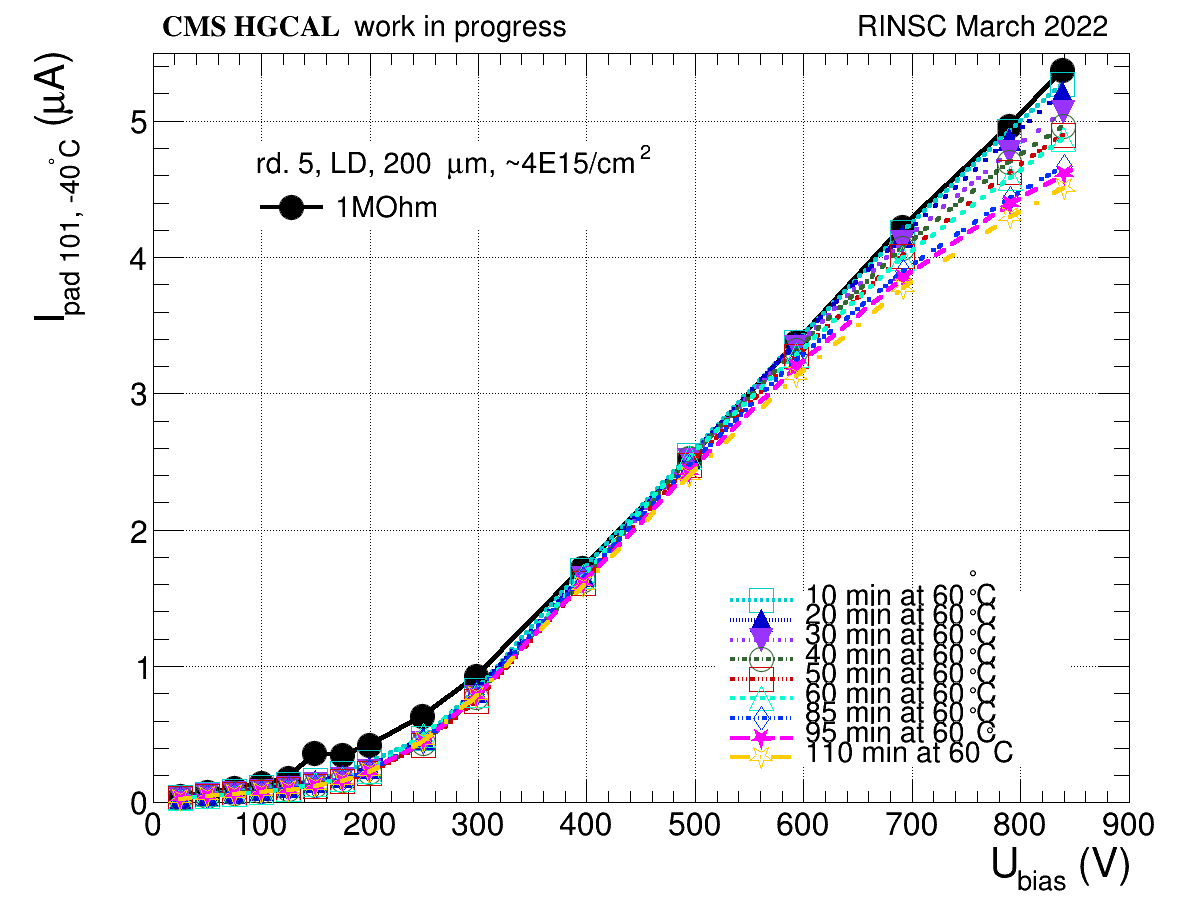
\includegraphics[width=1.0\textwidth]{plots/annealing_IV_ch101_N4790_21.png}
            \caption{Annealing effect on IV of pad 101}
        \end{figure}
        \column{.5\textwidth}
        \begin{figure}
            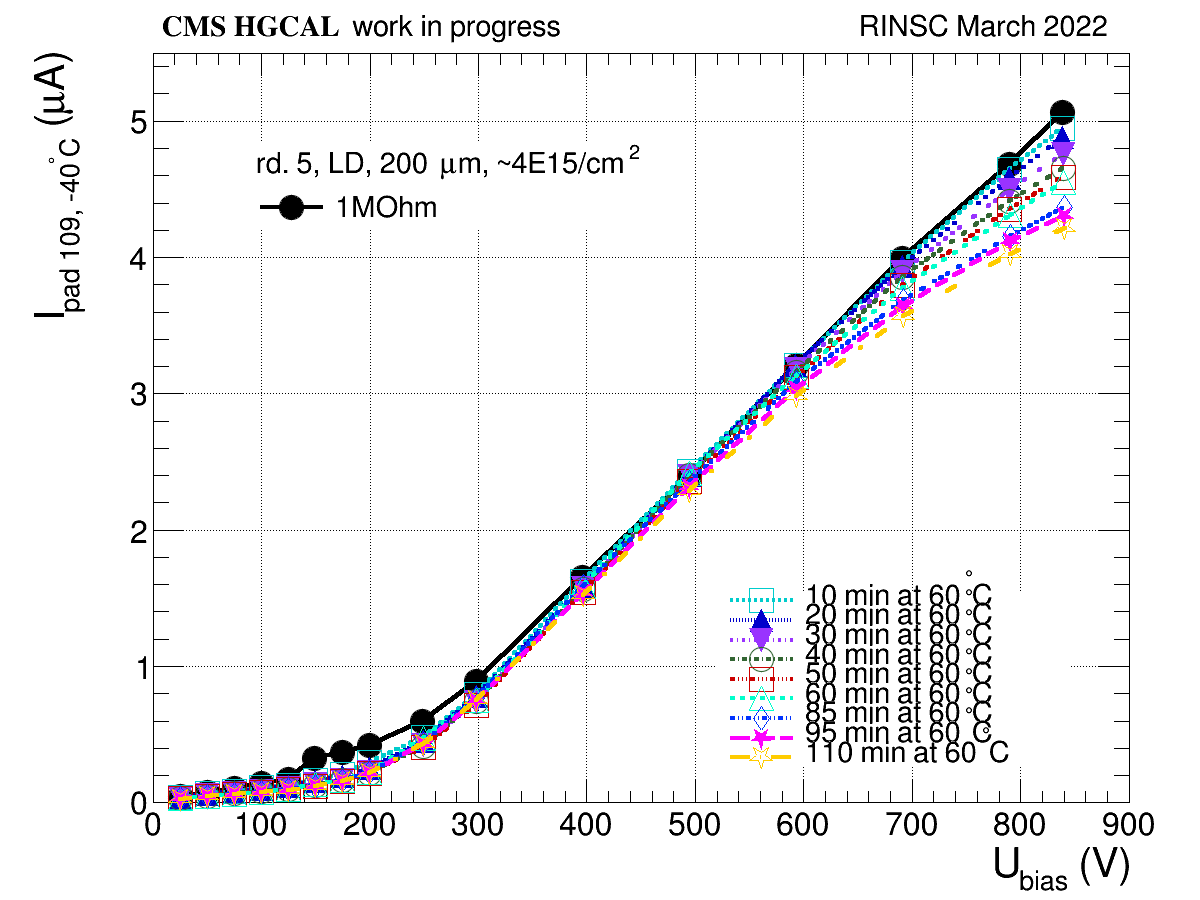
\includegraphics[width=1.0\textwidth]{plots/8in_198ch_2019_N4790_21_4E15_neg40degC_annealing_IV_ch109.png}
            \caption{Annealing effect on IV of pad 109}
        \end{figure}
    \end{columns}
    \begin{itemize}
        \item We do see annealing effect on current
        \item Annealing on IV results of other channels all consistent( backup)
    \end{itemize}
\end{frame}

\begin{frame}{Current vs annealing time for 600V and 650V}
  \begin{columns}
       \column{.5\textwidth}
       \begin{figure}
           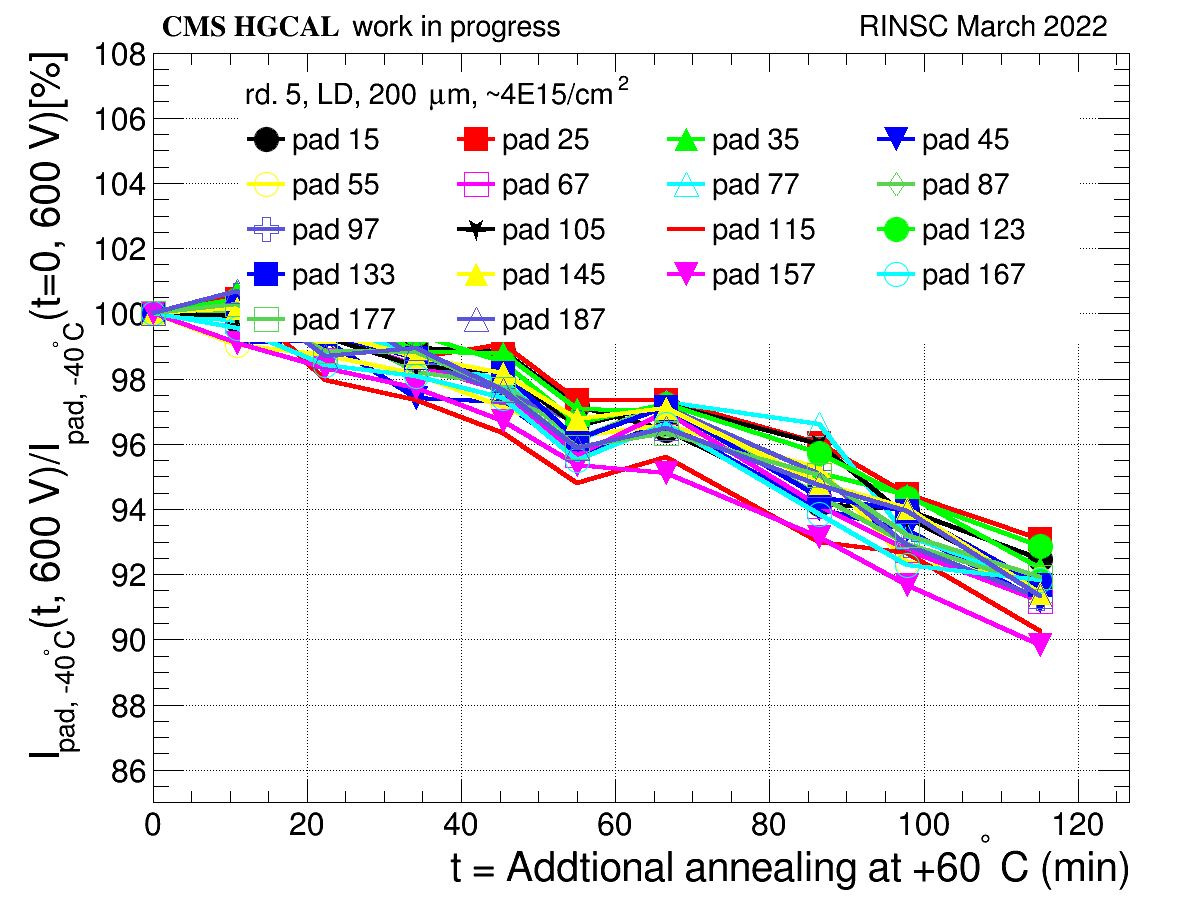
\includegraphics[width=1.0\textwidth]{plots/8in_198ch_2019_N4790_21_4E15_neg40degC_annealing_current_600.png}
       \end{figure}
       \column{.5\textwidth}
       \begin{figure}
           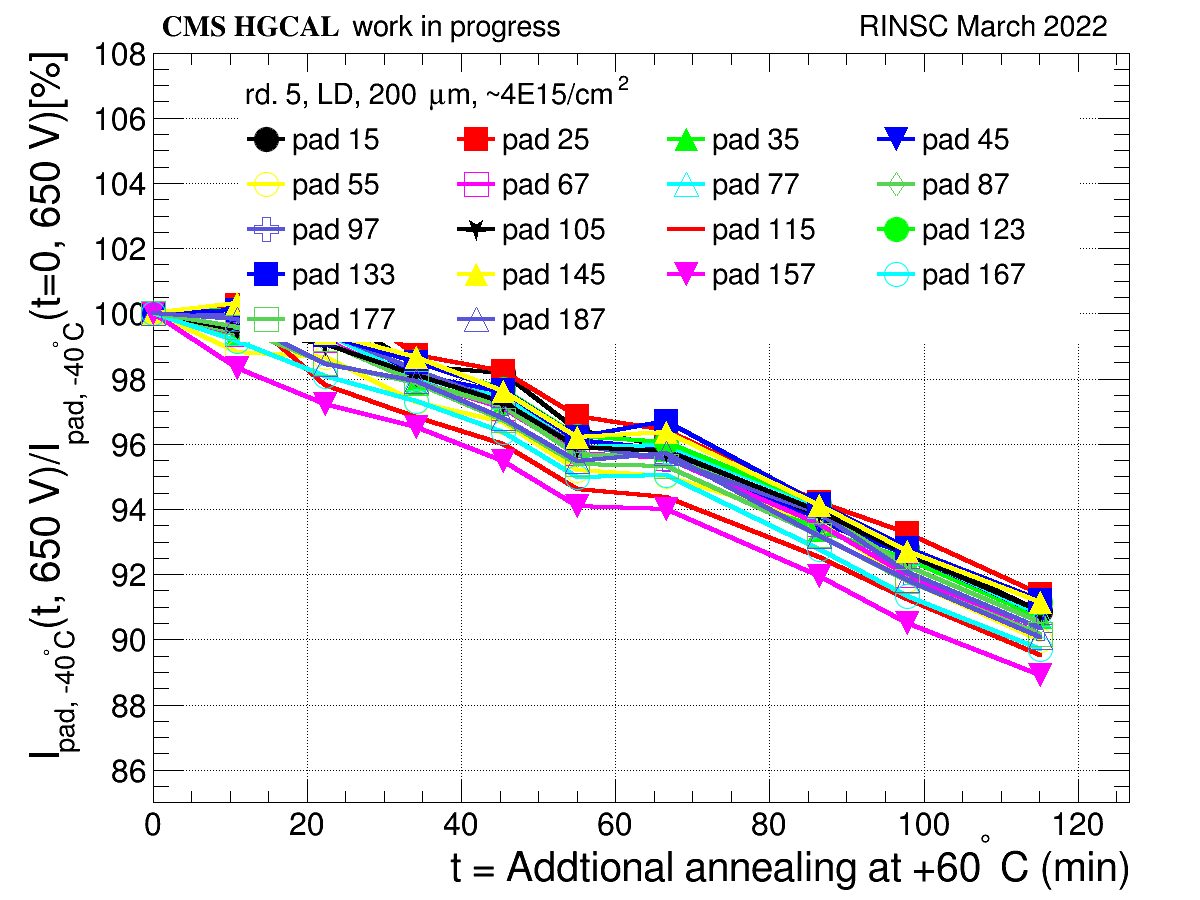
\includegraphics[width=1.0\textwidth]{plots/8in_198ch_2019_N4790_21_4E15_neg40degC_annealing_current_650.png}
       \end{figure}
   \end{columns}
\end{frame}

\begin{frame}{Current vs annealing time for 700V and 800V}
  \begin{columns}
       \column{.5\textwidth}
       \begin{figure}
           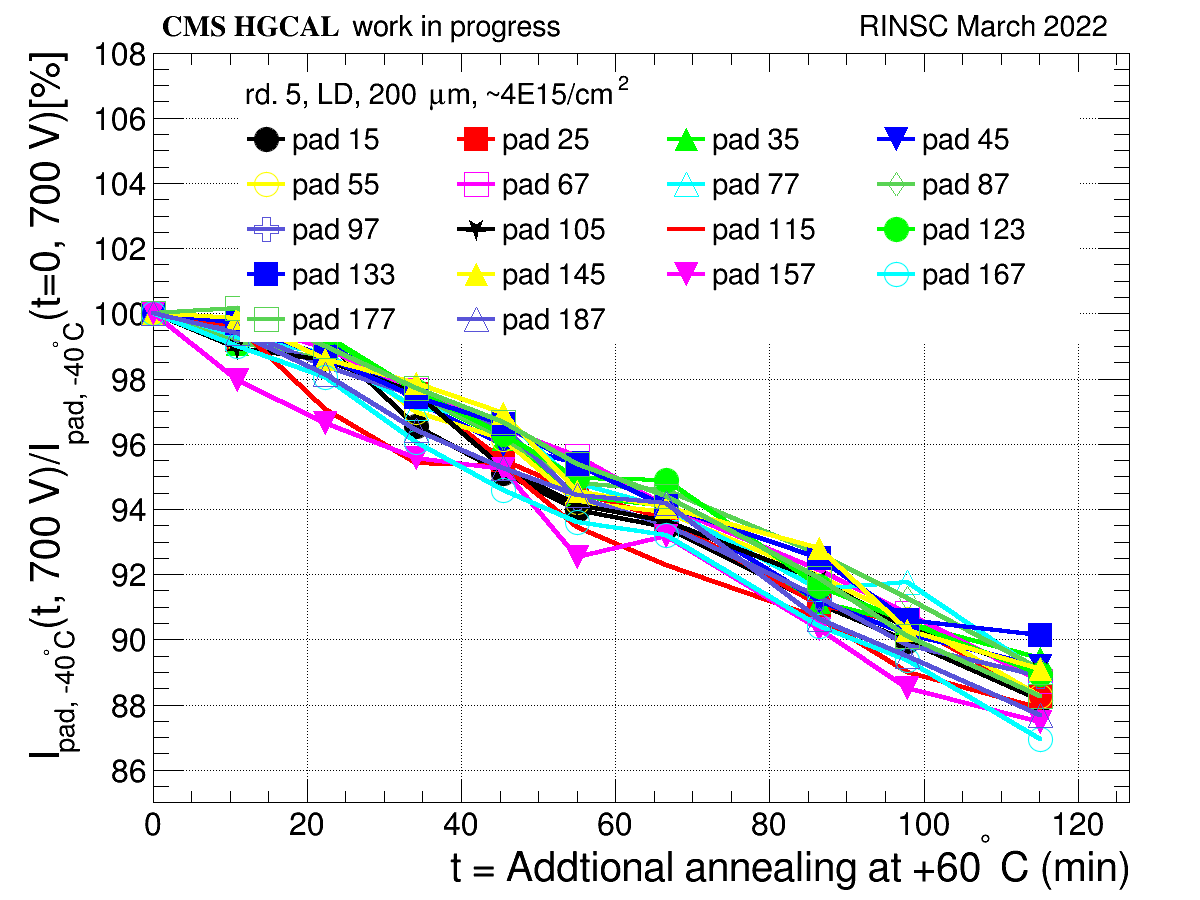
\includegraphics[width=1.0\textwidth]{plots/8in_198ch_2019_N4790_21_4E15_neg40degC_annealing_current_700.png}
       \end{figure}
       \column{.5\textwidth}
       \begin{figure}
           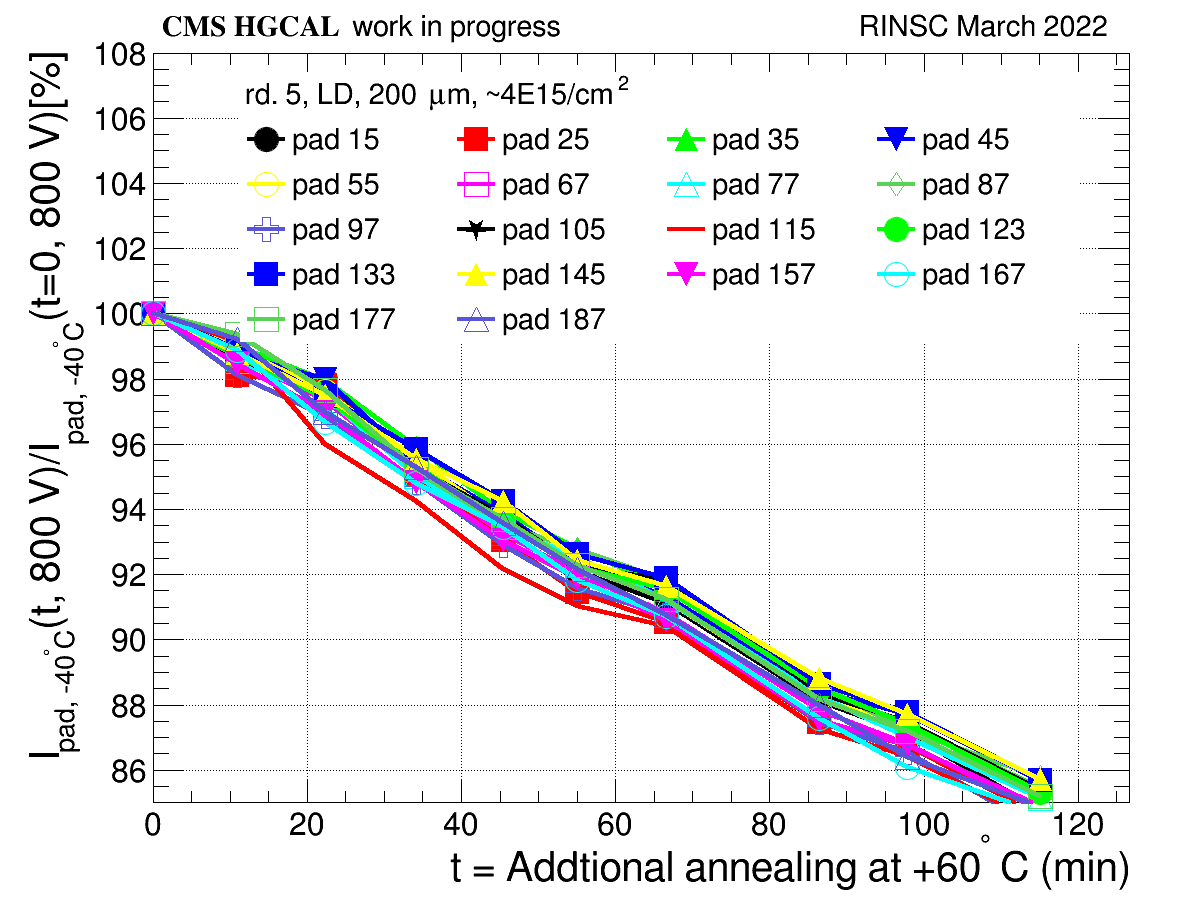
\includegraphics[width=1.0\textwidth]{plots/8in_198ch_2019_N4790_21_4E15_neg40degC_annealing_current_800.png}
       \end{figure}
   \end{columns}
\end{frame}

\subsection{N4790\_09}

\begin{frame}{Anealing effect on IV results(N4790\_09) }
  \begin{columns}
       \column{.5\textwidth}
       \begin{figure}
           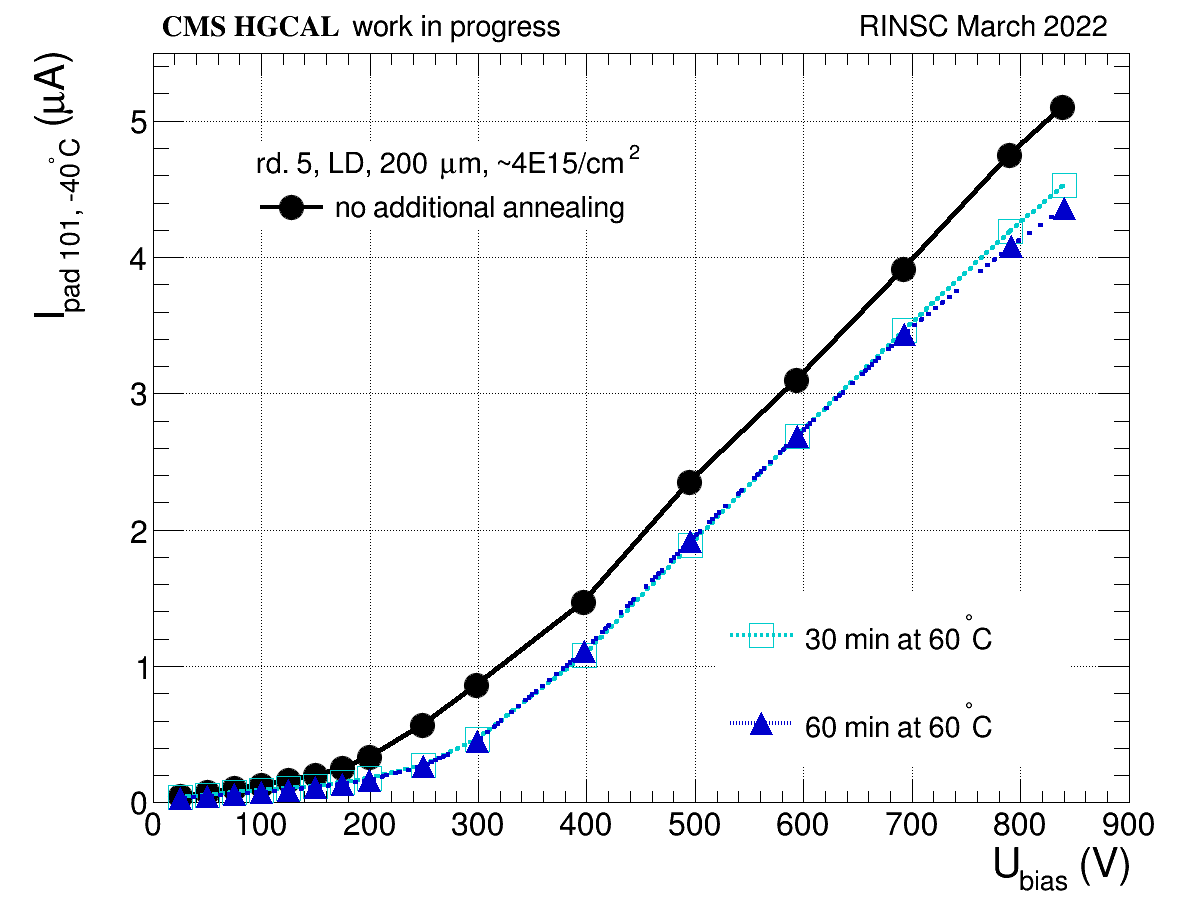
\includegraphics[width=1.0\textwidth]{plots/8in_198ch_2019_N4790_09_4E15_neg40degC_annealing_IV_ch101.png}
           \caption{Annealing effect on IV channel 101 }
       \end{figure}
       \column{.5\textwidth}
       \begin{figure}
           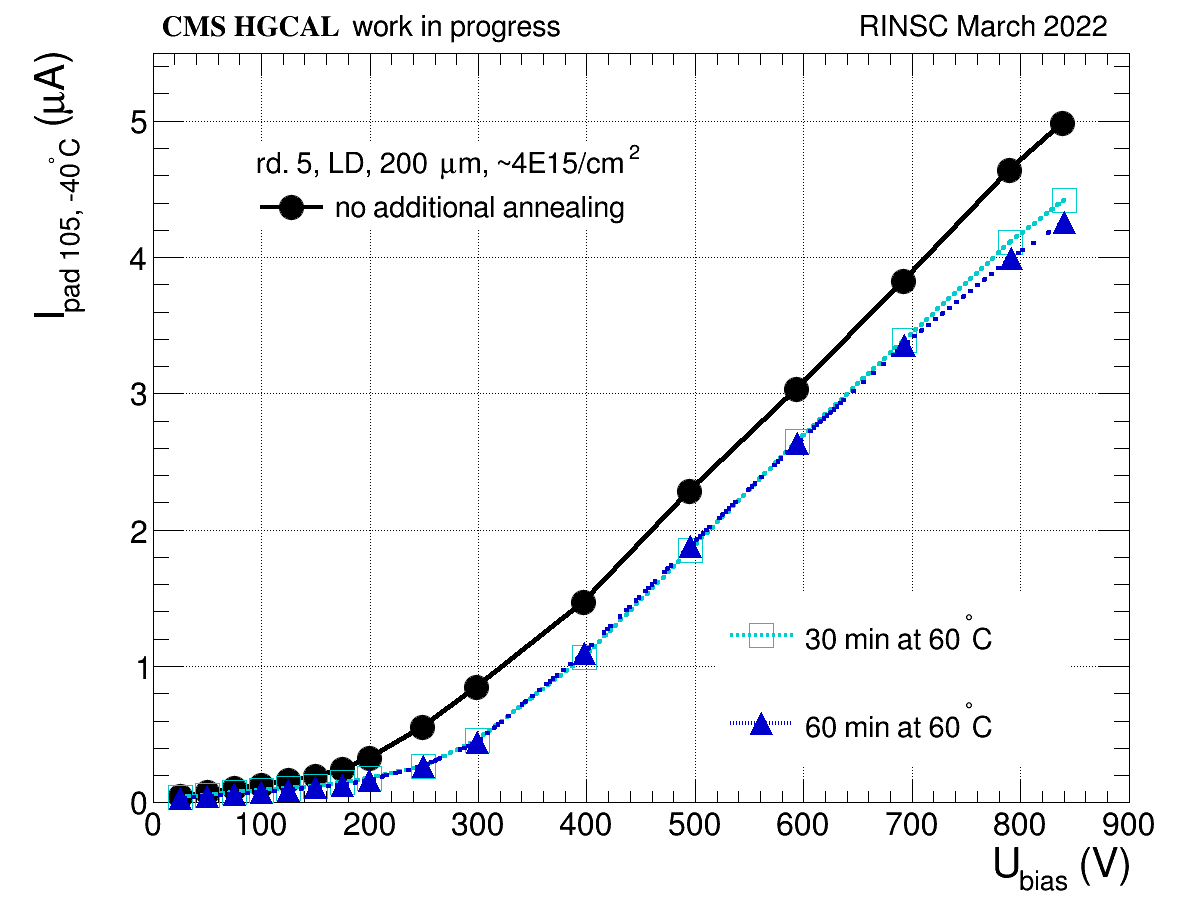
\includegraphics[width=1.0\textwidth]{plots/8in_198ch_2019_N4790_09_4E15_neg40degC_annealing_IV_ch105.png}
           \caption{Annealing effect on IV channel 105}
       \end{figure}
   \end{columns}
   \begin{itemize}
      \item Reached the limit at around 60 mins
      \item Other channels all have consistent plot(exeptions exist!)
   \end{itemize}
\end{frame}

\begin{frame}{Current vs annealing time for 600V and 650V}
  \begin{columns}
       \column{.5\textwidth}
       \begin{figure}
           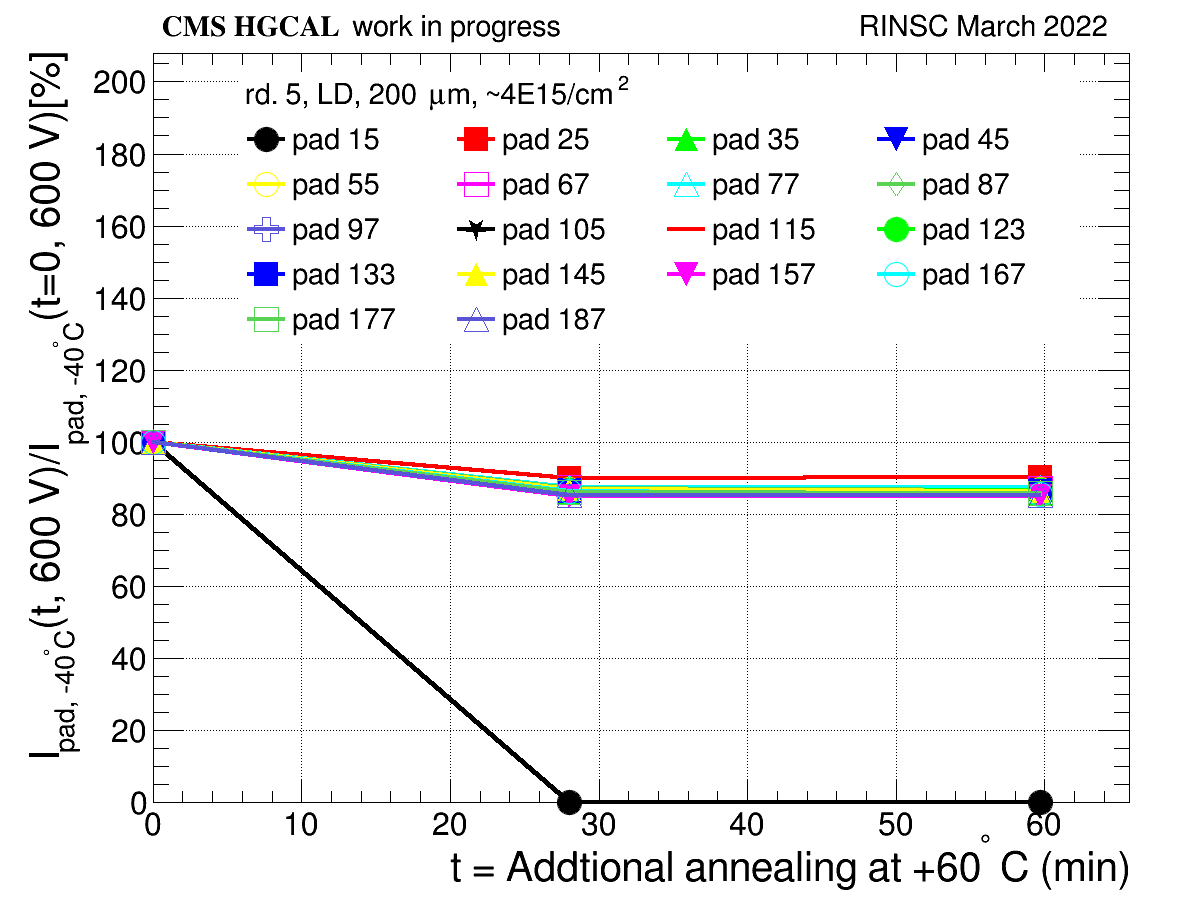
\includegraphics[width=1.0\textwidth]{plots/8in_198ch_2019_N4790_09_4E15_neg40degC_annealing_current_600.png}
       \end{figure}
       \column{.5\textwidth}
       \begin{figure}
           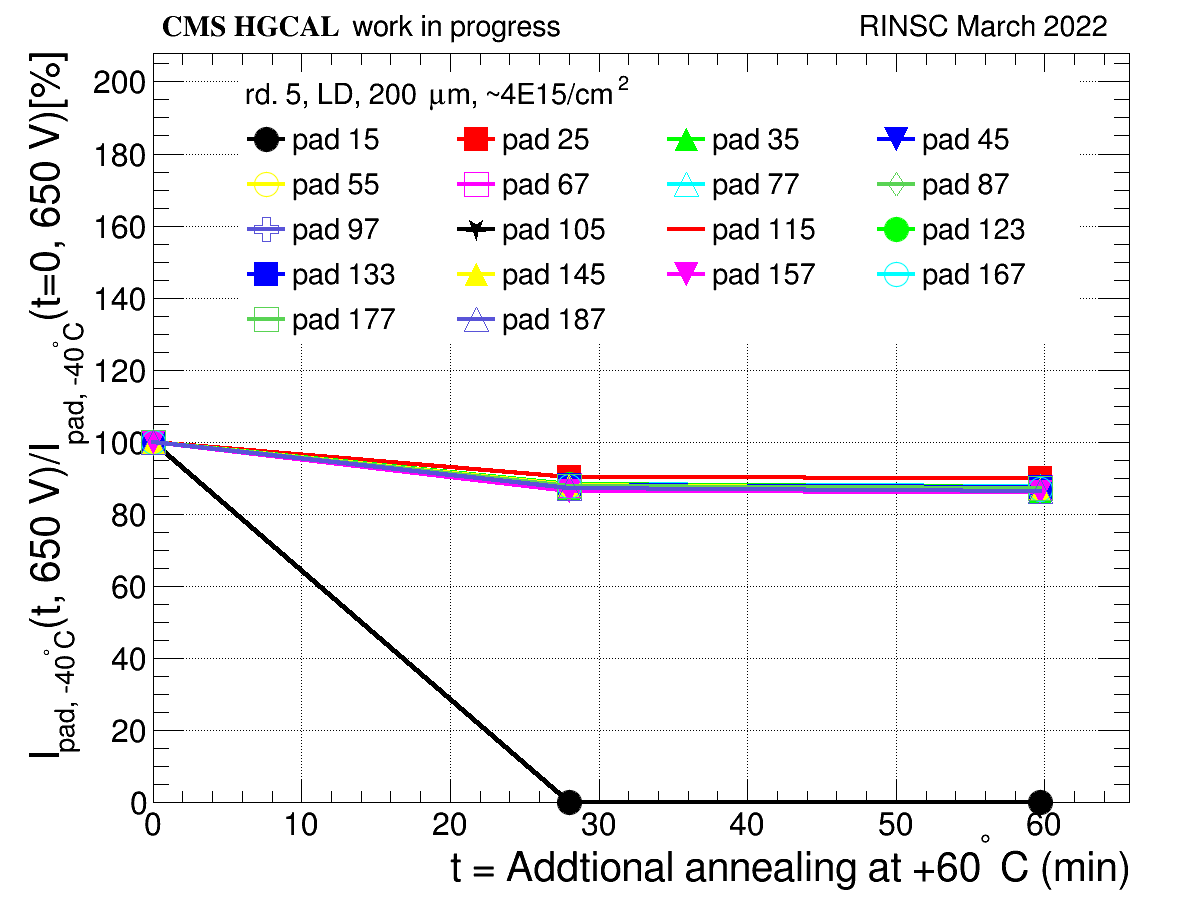
\includegraphics[width=1.0\textwidth]{plots/8in_198ch_2019_N4790_09_4E15_neg40degC_annealing_current_650.png}
       \end{figure}
   \end{columns}
   \begin{itemize}
      \item Channel 15 seems to be masked at 30 and 60 annealing measurement
     \item Only drawing 18 channels, there could be more abnormal channels like 15
     \item Need to further investigate this
   \end{itemize}
\end{frame}

\begin{frame}{Current vs annealing time for 700V and 800V}
  \begin{columns}
       \column{.5\textwidth}
       \begin{figure}
           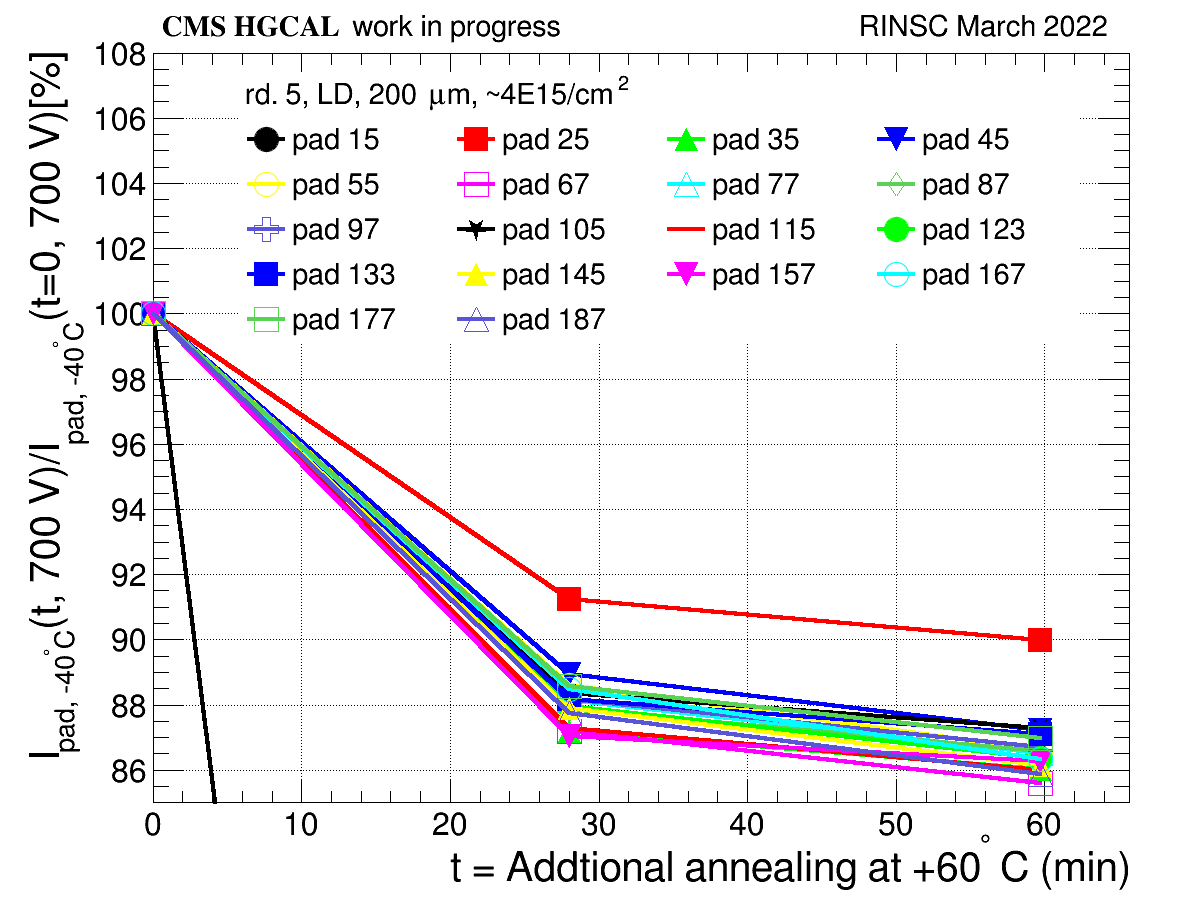
\includegraphics[width=1.0\textwidth]{plots/8in_198ch_2019_N4790_09_4E15_neg40degC_annealing_current_700.png}
       \end{figure}
       \column{.5\textwidth}
       \begin{figure}
           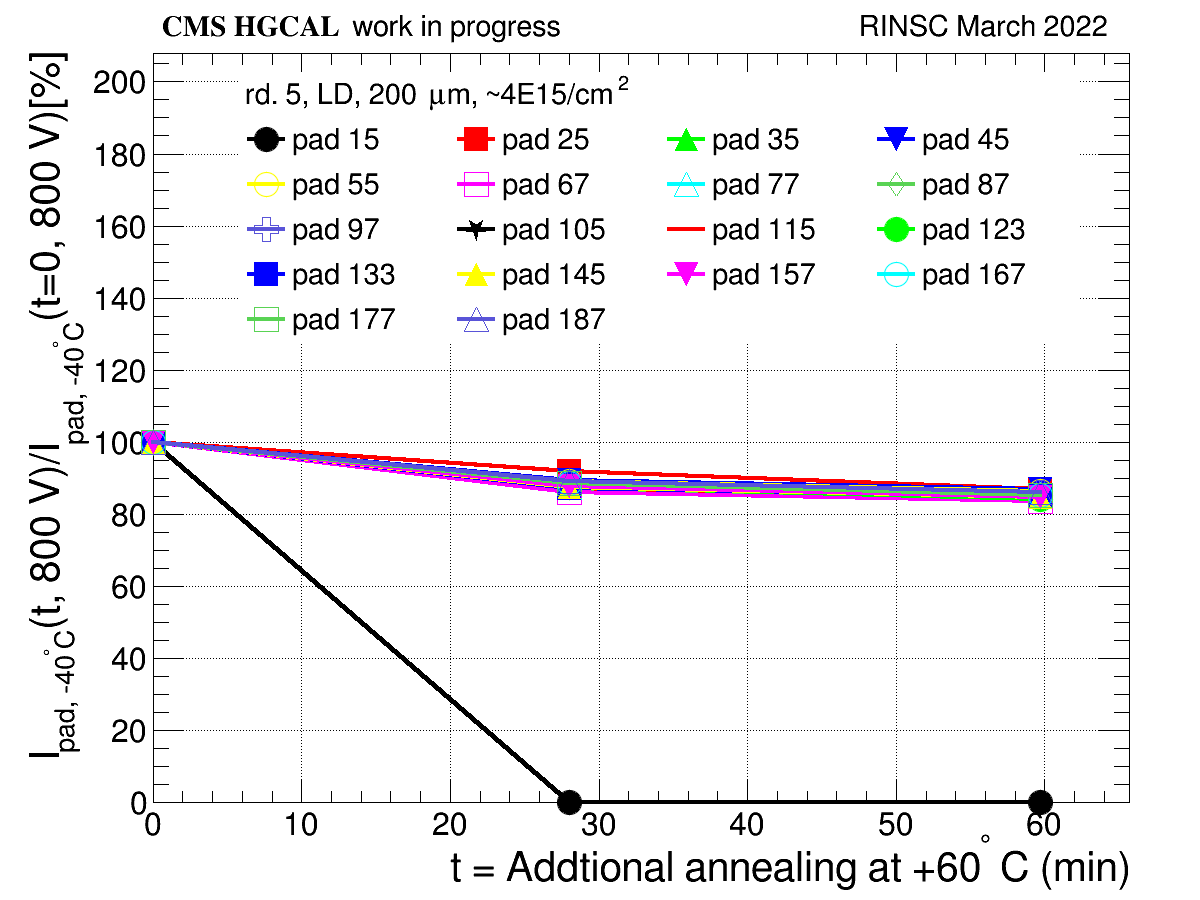
\includegraphics[width=1.0\textwidth]{plots/8in_198ch_2019_N4790_09_4E15_neg40degC_annealing_current_800.png}
       \end{figure}
   \end{columns}
\end{frame}

\begin{frame}{Anealing effect on IV channel 15 }
  \begin{columns}
       \column{.5\textwidth}
       \begin{figure}
           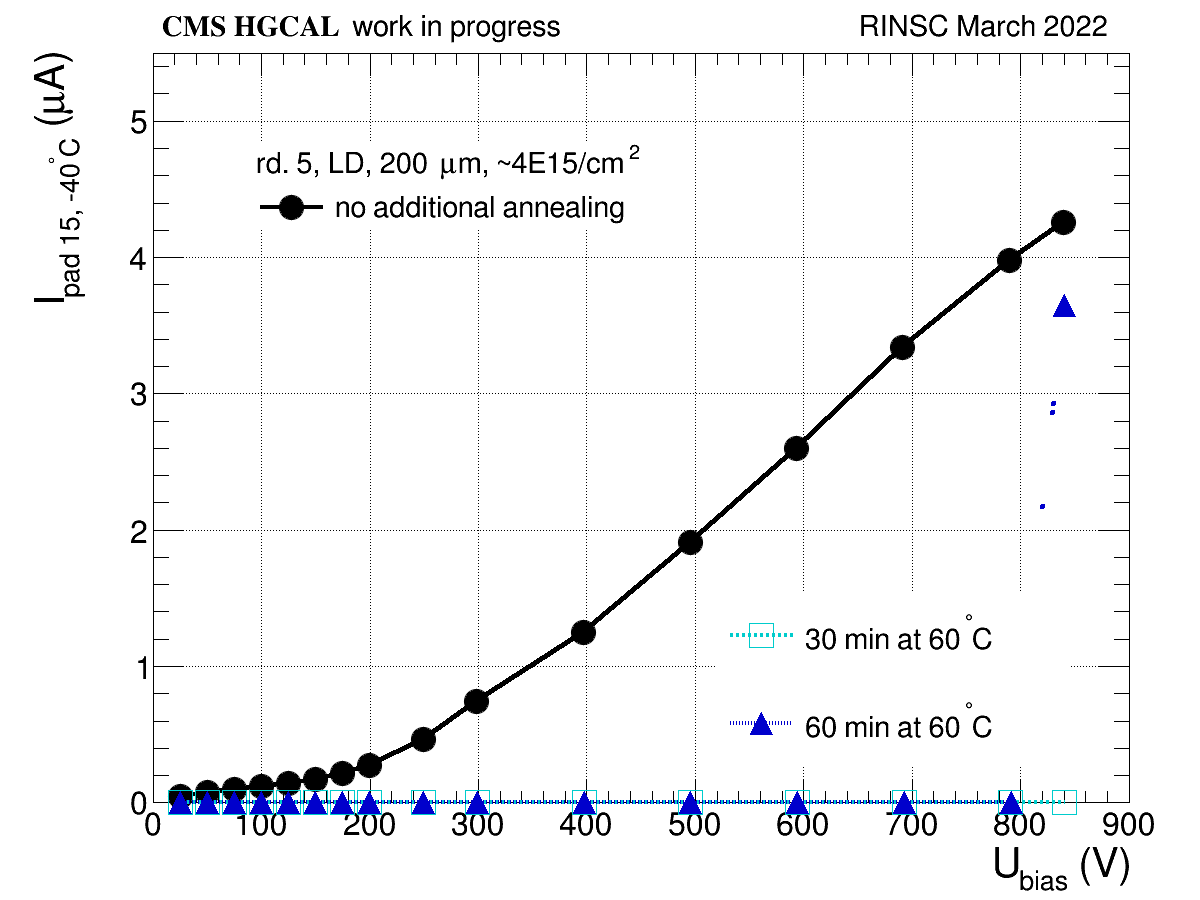
\includegraphics[width=1.0\textwidth]{plots/8in_198ch_2019_N4790_09_4E15_neg40degC_annealing_IV_ch15.png}
           \caption{Annealing effect on IV channel 15 }
       \end{figure}
       \column{.5\textwidth}
       \begin{figure}
           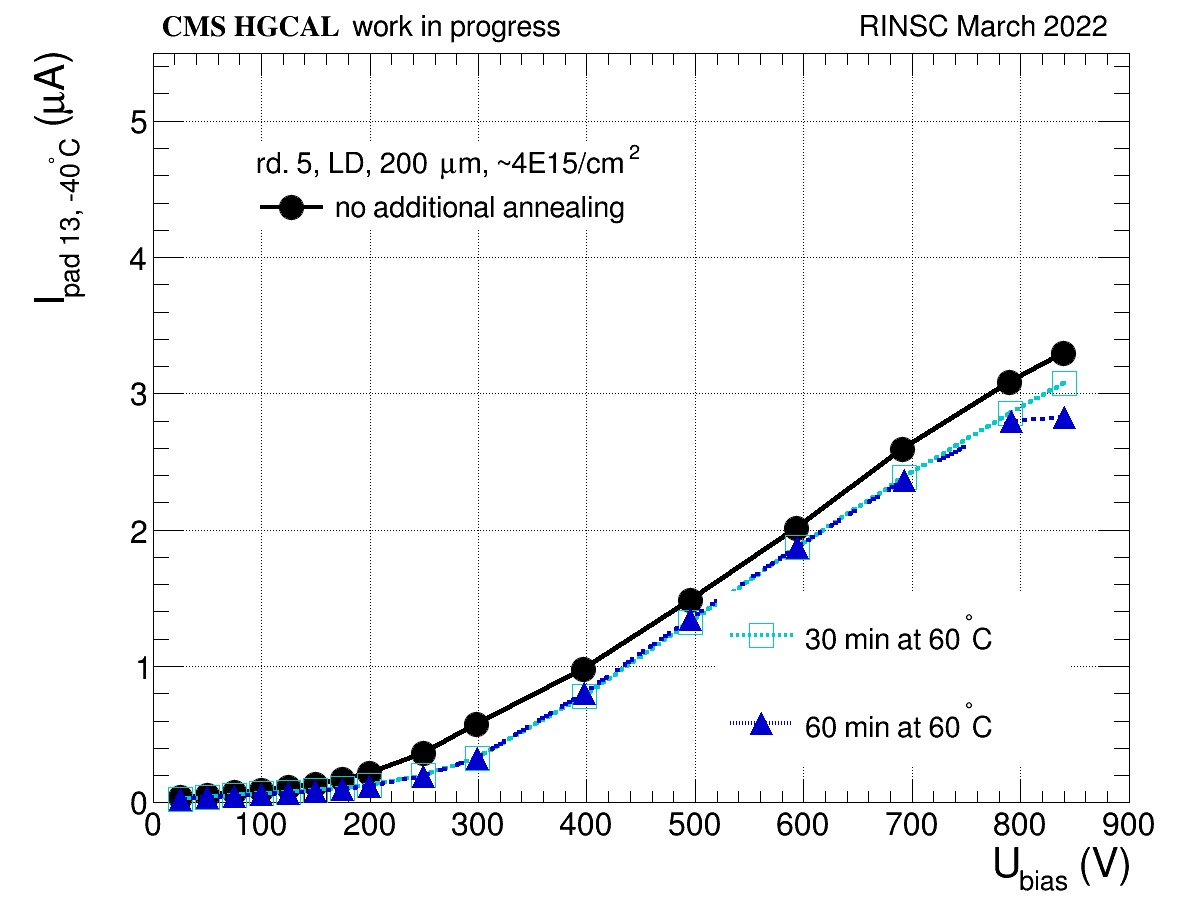
\includegraphics[width=1.0\textwidth]{plots/8in_198ch_2019_N4790_09_4E15_neg40degC_annealing_IV_ch13.png}
           \caption{Annealing effect on IV channel 13}
       \end{figure}
   \end{columns}
\end{frame}



\subsection{N4792\_07}

\begin{frame}{Anealing effect on IV results(N4792\_07 }
  \begin{columns}
       \column{.5\textwidth}
       \begin{figure}
           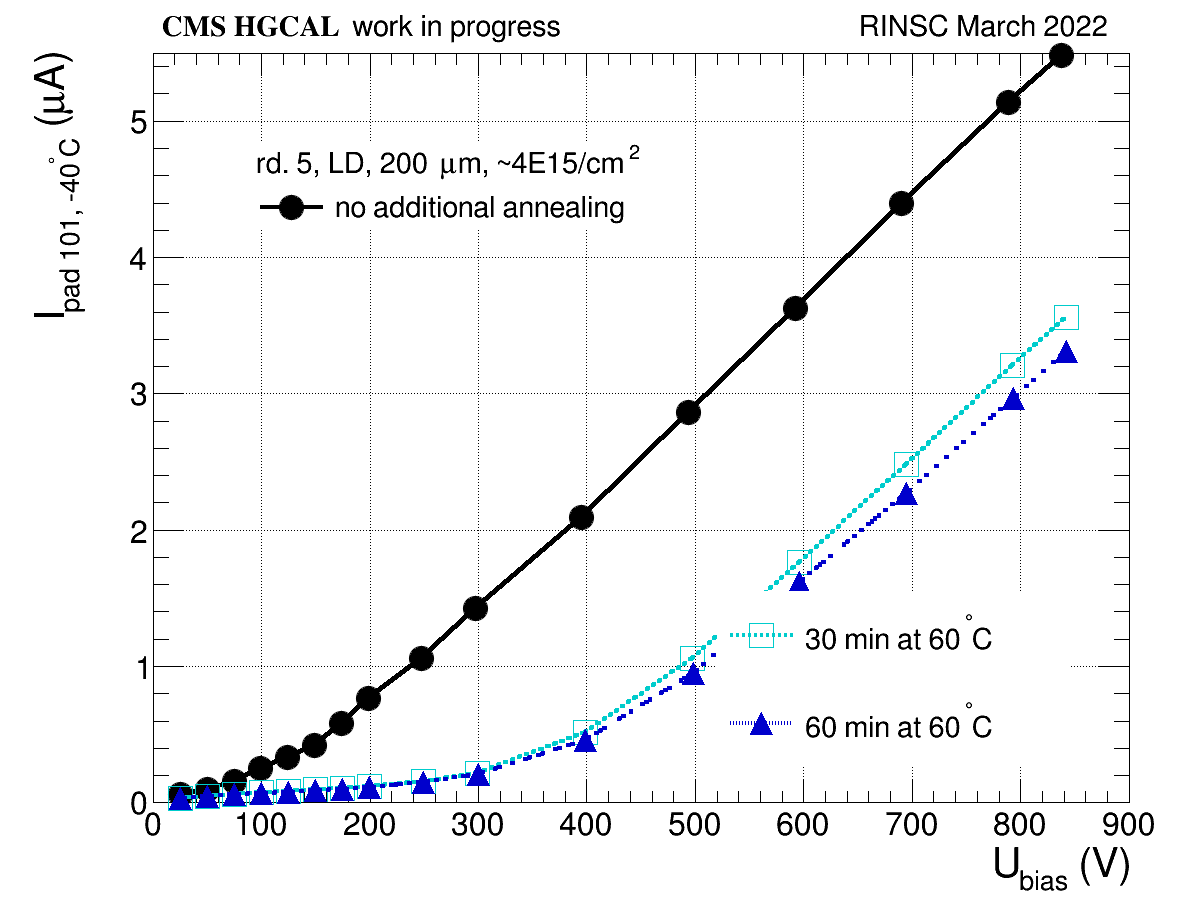
\includegraphics[width=1.0\textwidth]{plots/8in_198ch_2019_N4792_7_neg40degC_annealing_IV_ch101.png}
           \caption{Annealing effect on IV channel 101 }
       \end{figure}
       \column{.5\textwidth}
       \begin{figure}
           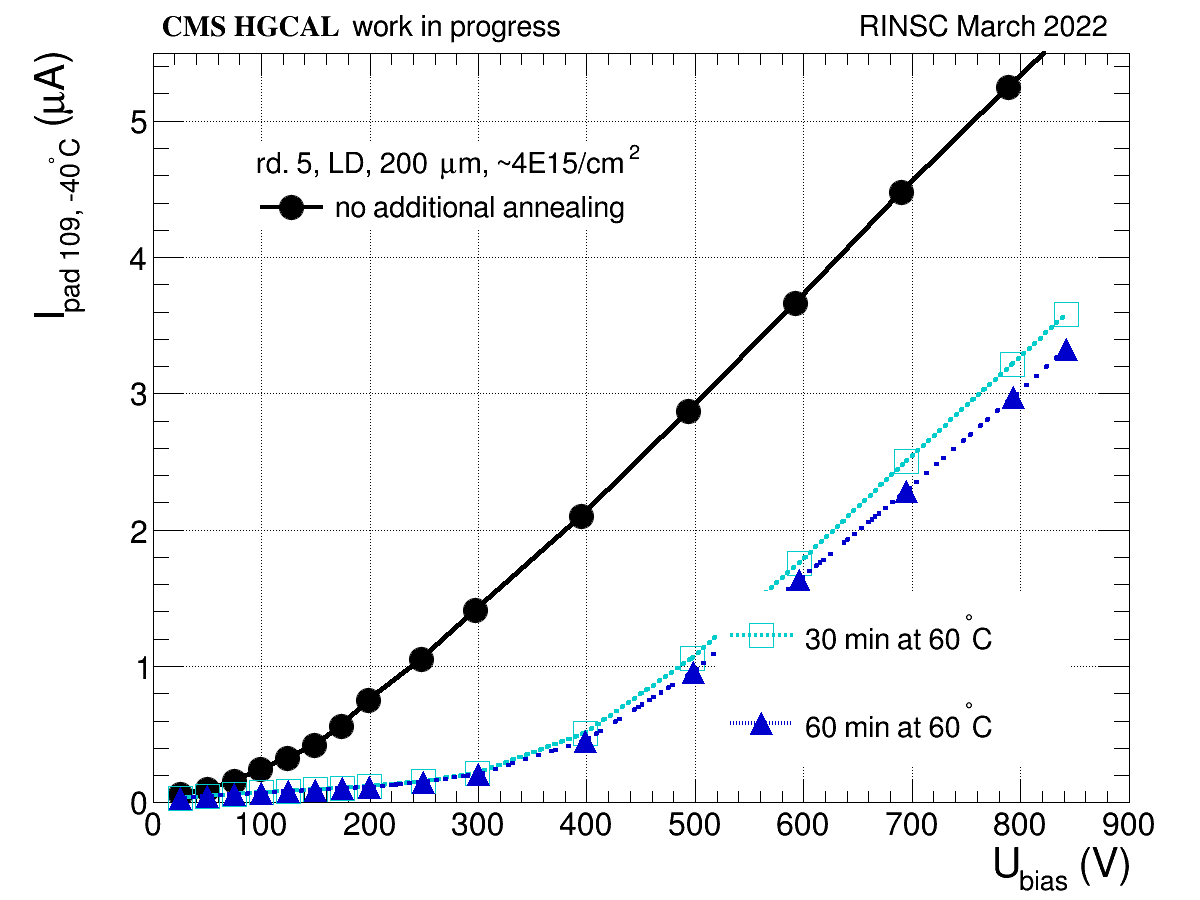
\includegraphics[width=1.0\textwidth]{plots/8in_198ch_2019_N4792_7_neg40degC_annealing_IV_ch109.png}
           \caption{Annealing effect on IV channel 109}
       \end{figure}
   \end{columns}
   \begin{itemize}
    \item Current drop is significantly higher than for other sensors
      \item Maybe reached the limit at around 60 mins
      \item Other channels all have consistent plot
   \end{itemize}
\end{frame}

\begin{frame}{Current vs annealing time for 600V and 650V}
  \begin{columns}
       \column{.5\textwidth}
       \begin{figure}
           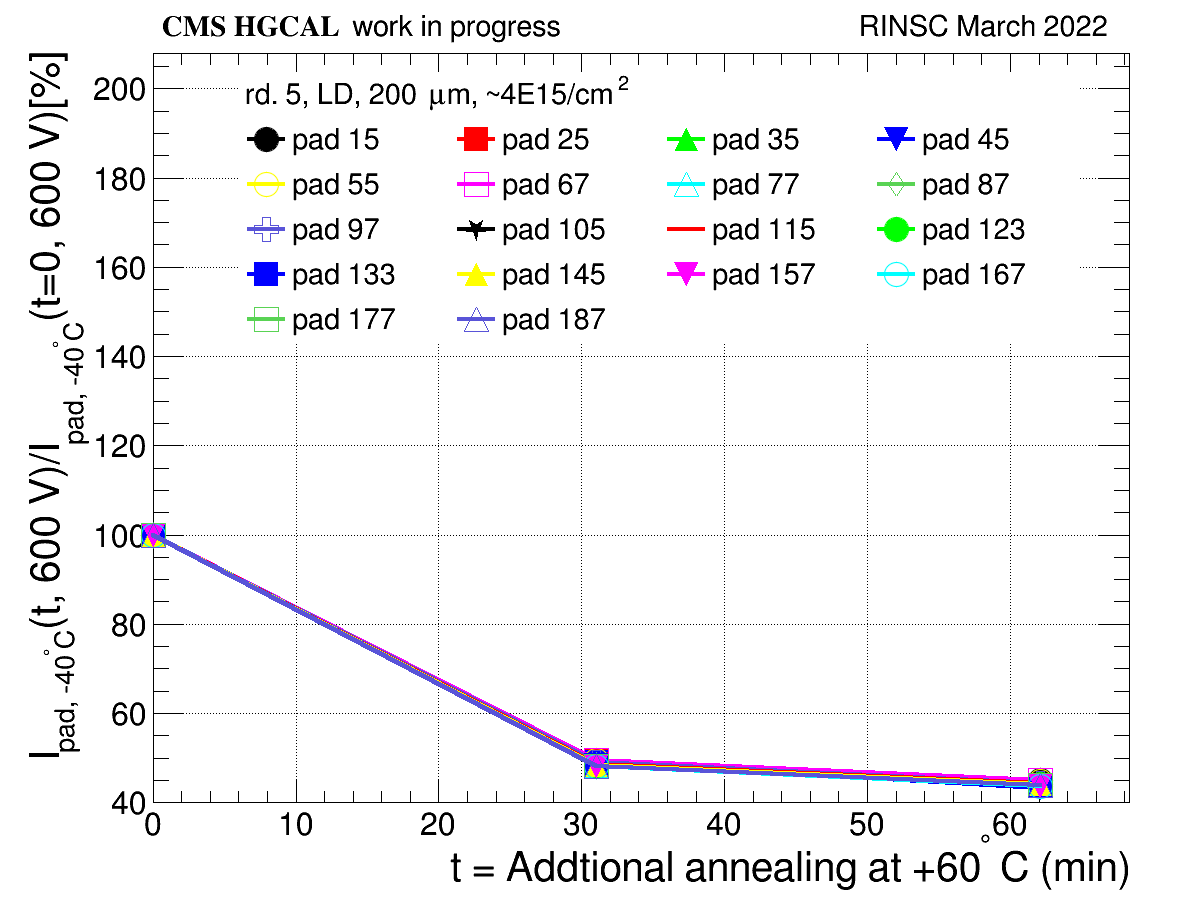
\includegraphics[width=1.0\textwidth]{plots/8in_198ch_2019_N4792_7_neg40degC_annealing_current_600.png}
       \end{figure}
       \column{.5\textwidth}
       \begin{figure}
           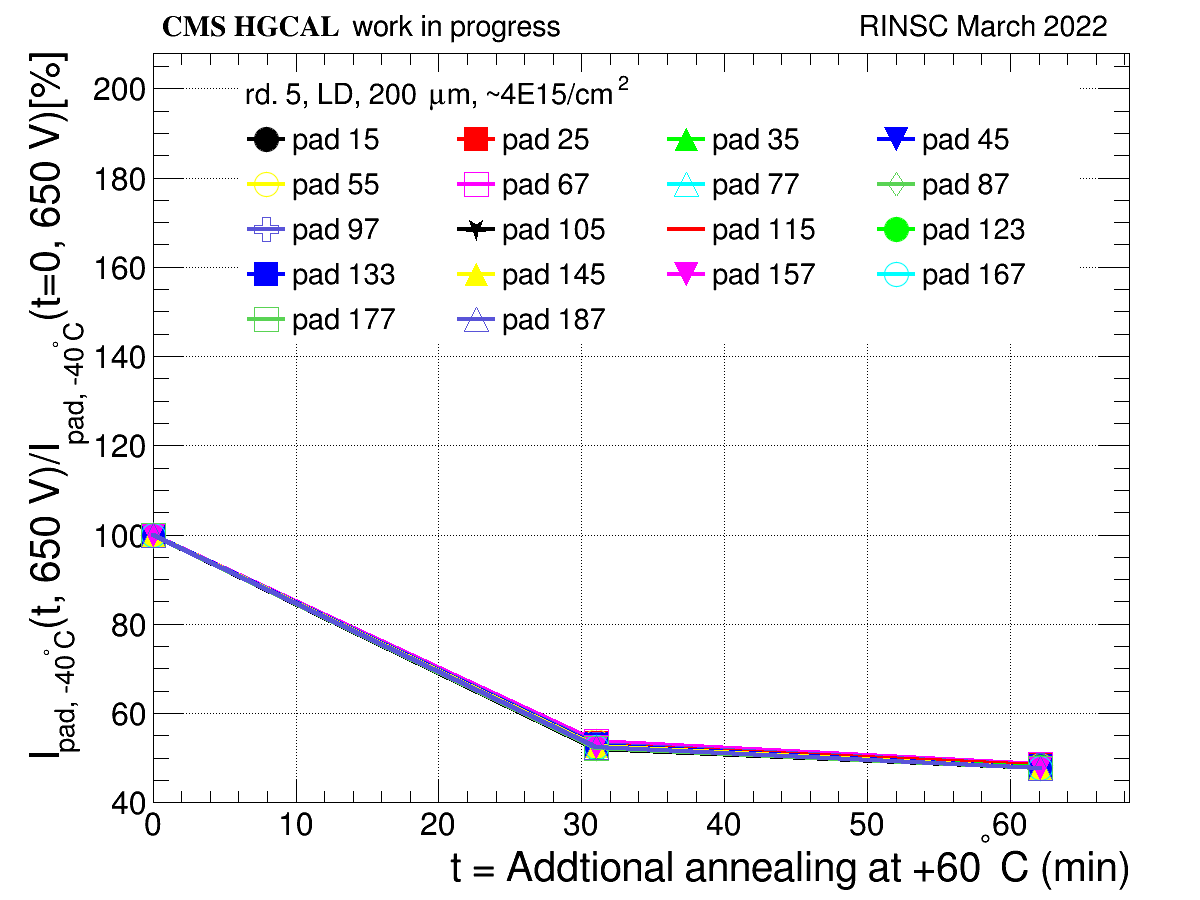
\includegraphics[width=1.0\textwidth]{plots/8in_198ch_2019_N4792_7_neg40degC_annealing_current_650.png}
       \end{figure}
   \end{columns}
   \begin{itemize}
    \item seems too good?
   \end{itemize}
\end{frame}


\section{Temperature effect}

\begin{frame}{Temperation effect on IV measurement}
    \begin{columns}
        \column{.5\textwidth}
        \begin{figure}
            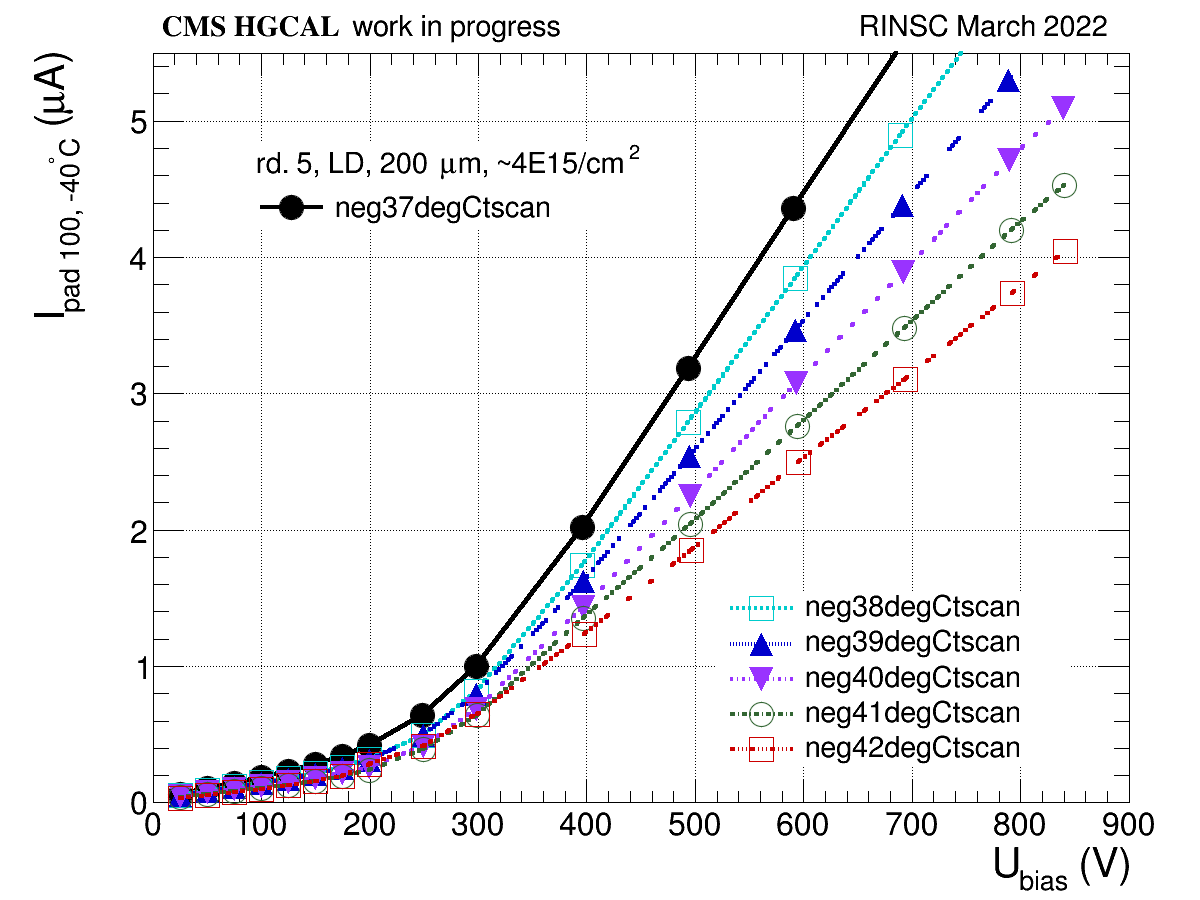
\includegraphics[width=1.0\textwidth]{plots/8in_198ch_2019_N4790_21_4E15_tempareture_effect_100.png}
        \end{figure}
        \column{.5\textwidth}
        \begin{figure}
            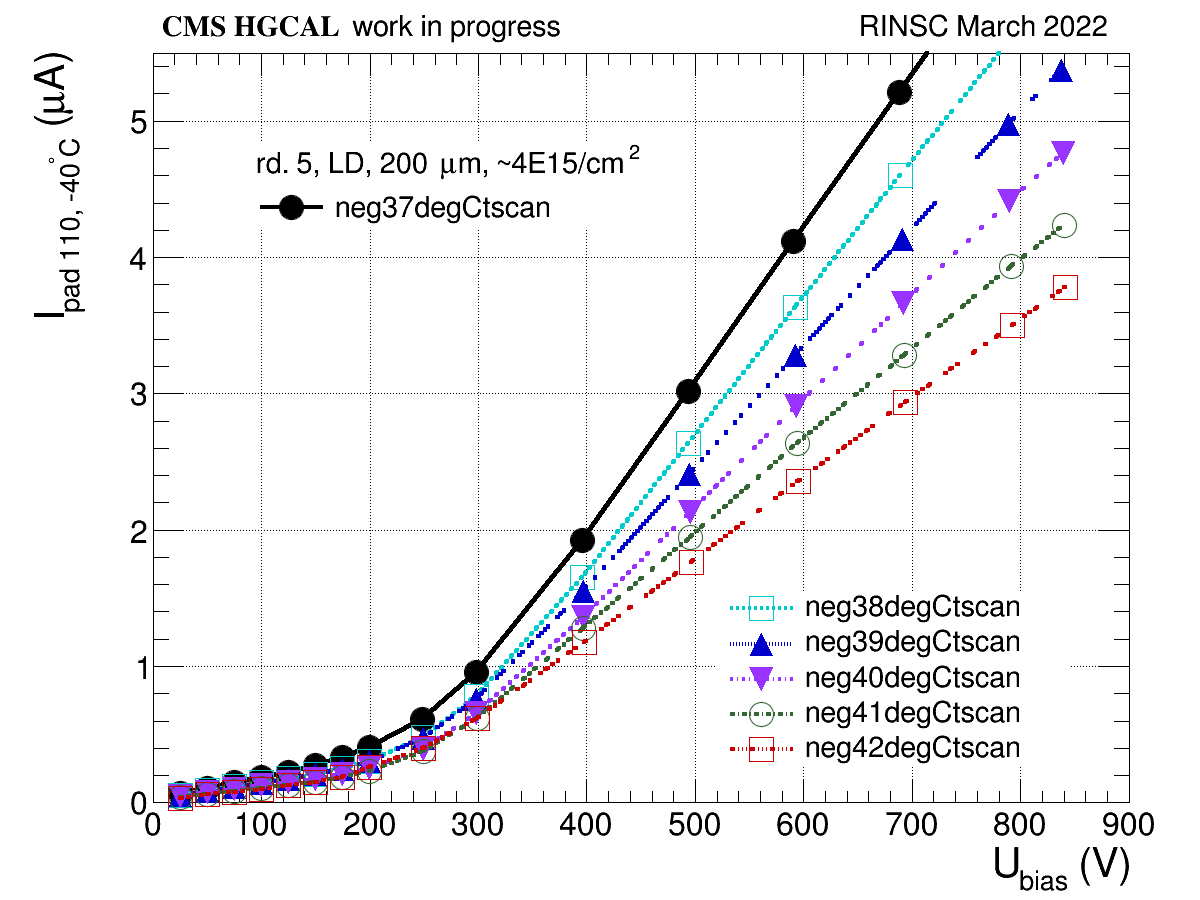
\includegraphics[width=1.0\textwidth]{plots/8in_198ch_2019_N4790_21_4E15_tempareture_effect_110.png}
        \end{figure}
    \end{columns}
\end{frame}




\subsection{IV Hexplots}

\begin{frame}{IV HexPlots}
  \begin{columns}
    \column{.33\textwidth}
    \begin{figure}
      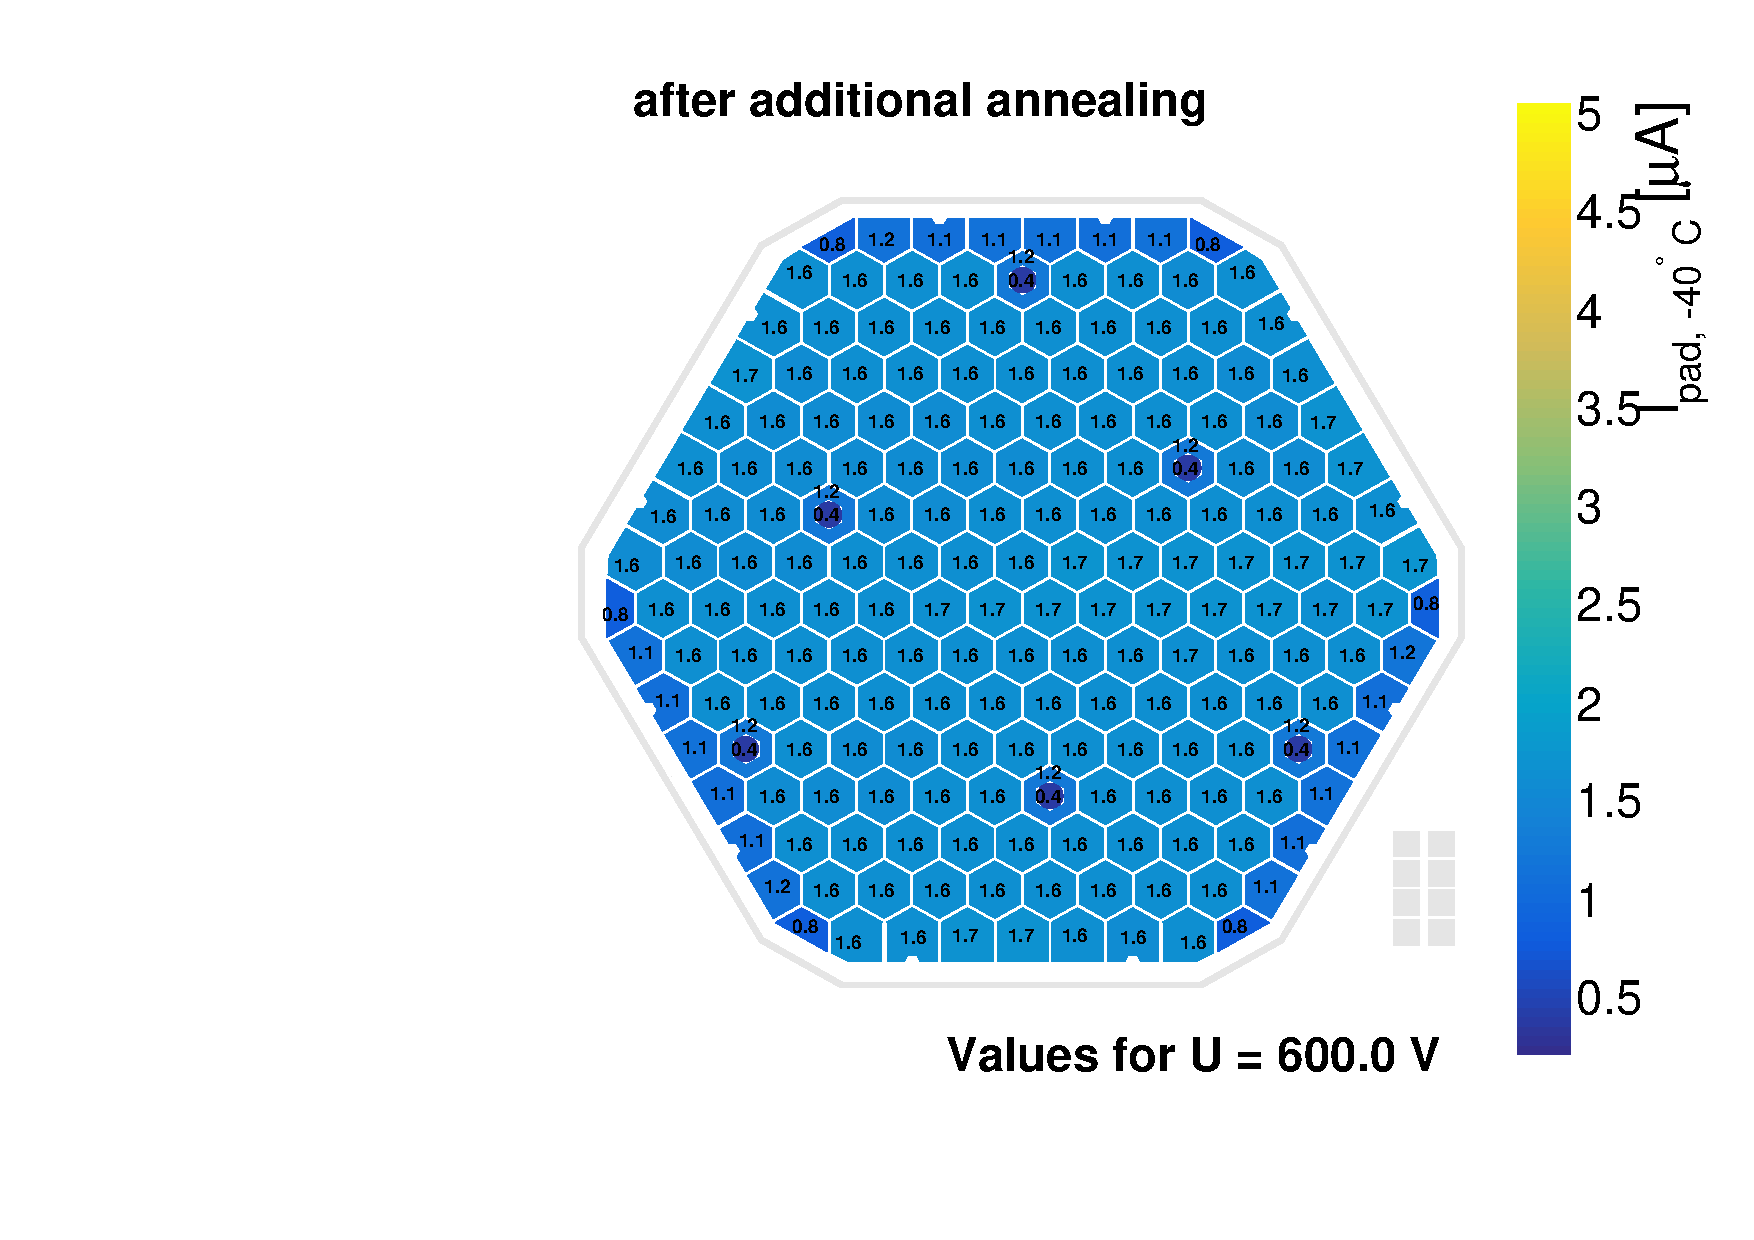
\includegraphics[width=0.7\textwidth]{plots/N4792_7.pdf}
      \caption{Round5, N4792\_7}
    \end{figure}

    \begin{figure}
      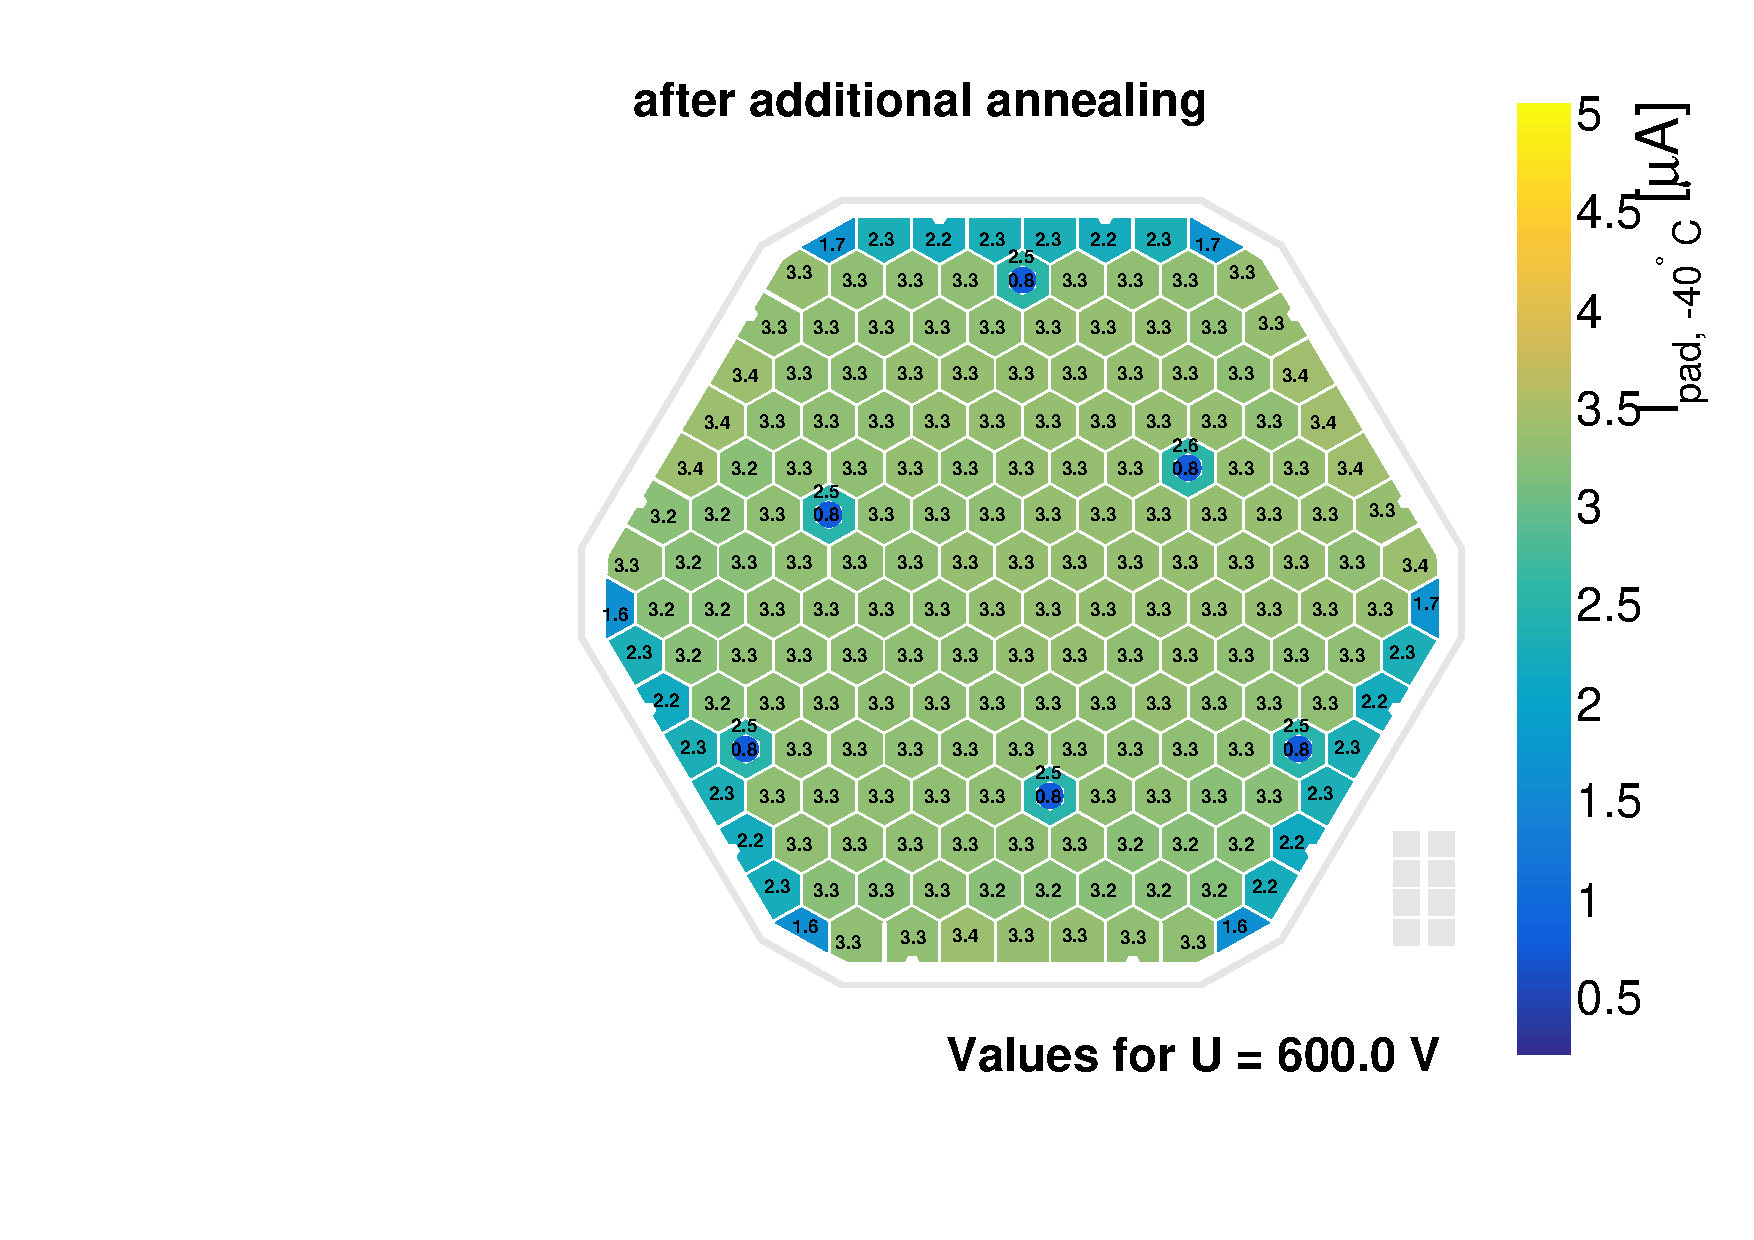
\includegraphics[width=0.7\textwidth]{plots/N4792_09.pdf}
      \caption{Round6, N4792\_09}
    \end{figure}


    \column{.33\textwidth}
    \begin{figure}
      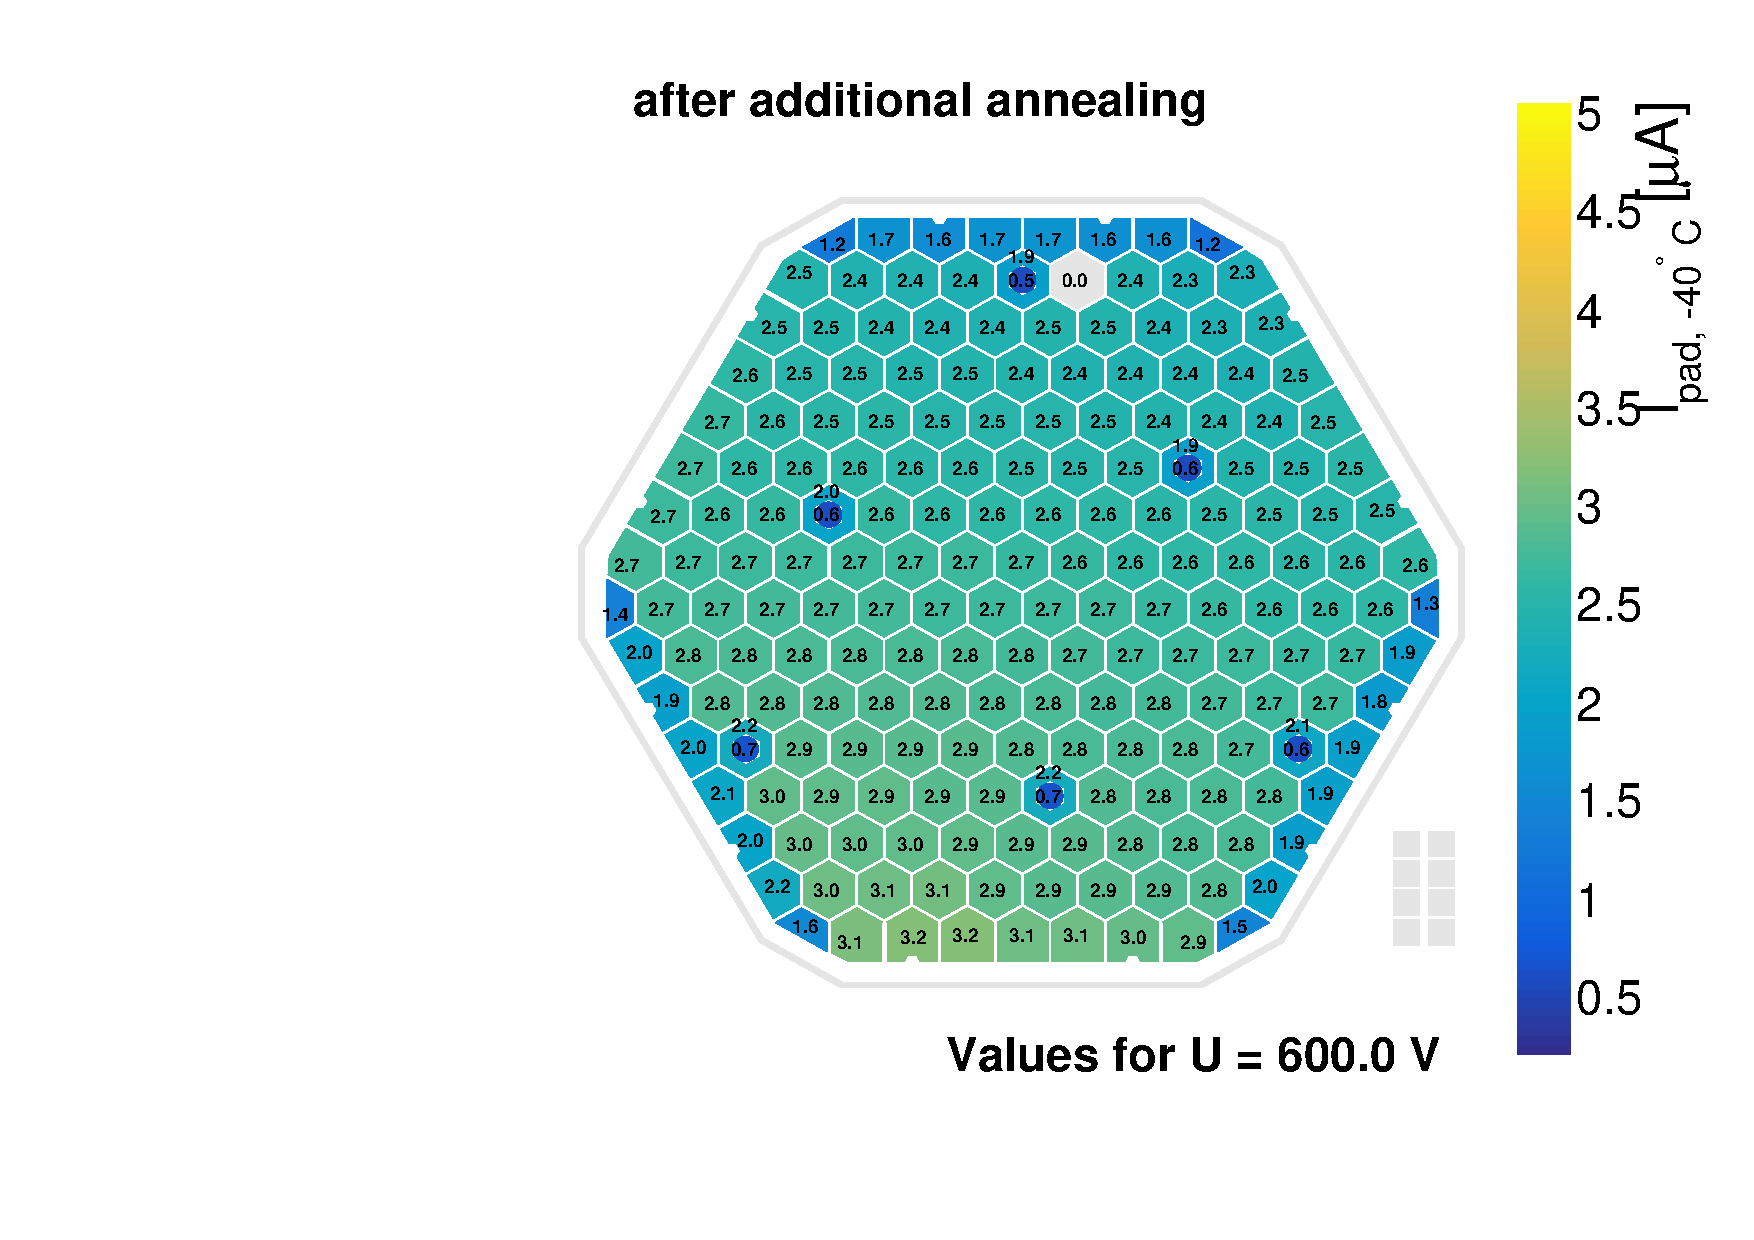
\includegraphics[width=0.7\textwidth]{plots/N4790_09.pdf}
      \caption{Round5, N4790\_09}
    \end{figure}

    \begin{figure}
      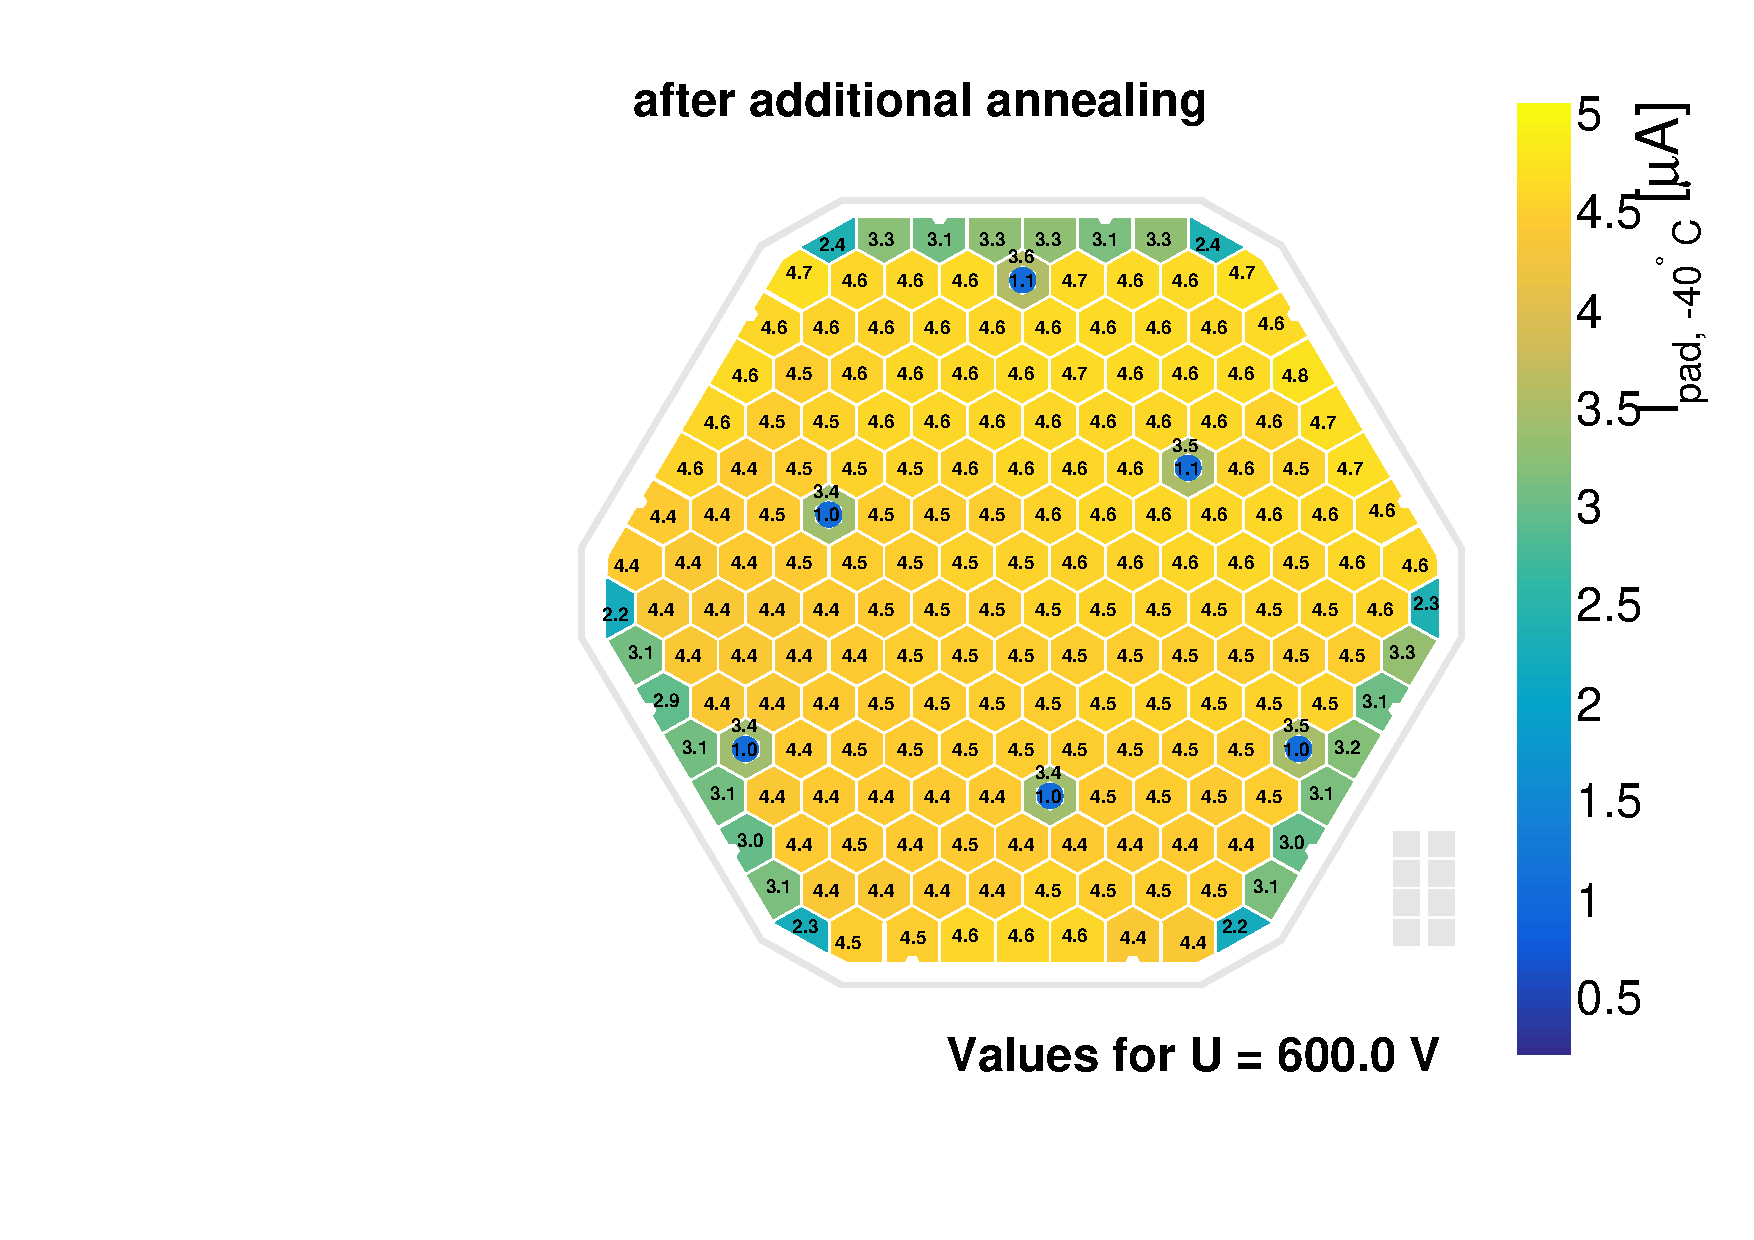
\includegraphics[width=0.7\textwidth]{plots/N4790_8.pdf}
      \caption{Round6, N4790\_8}
    \end{figure}

    \column{.33\textwidth}
    \begin{figure}
      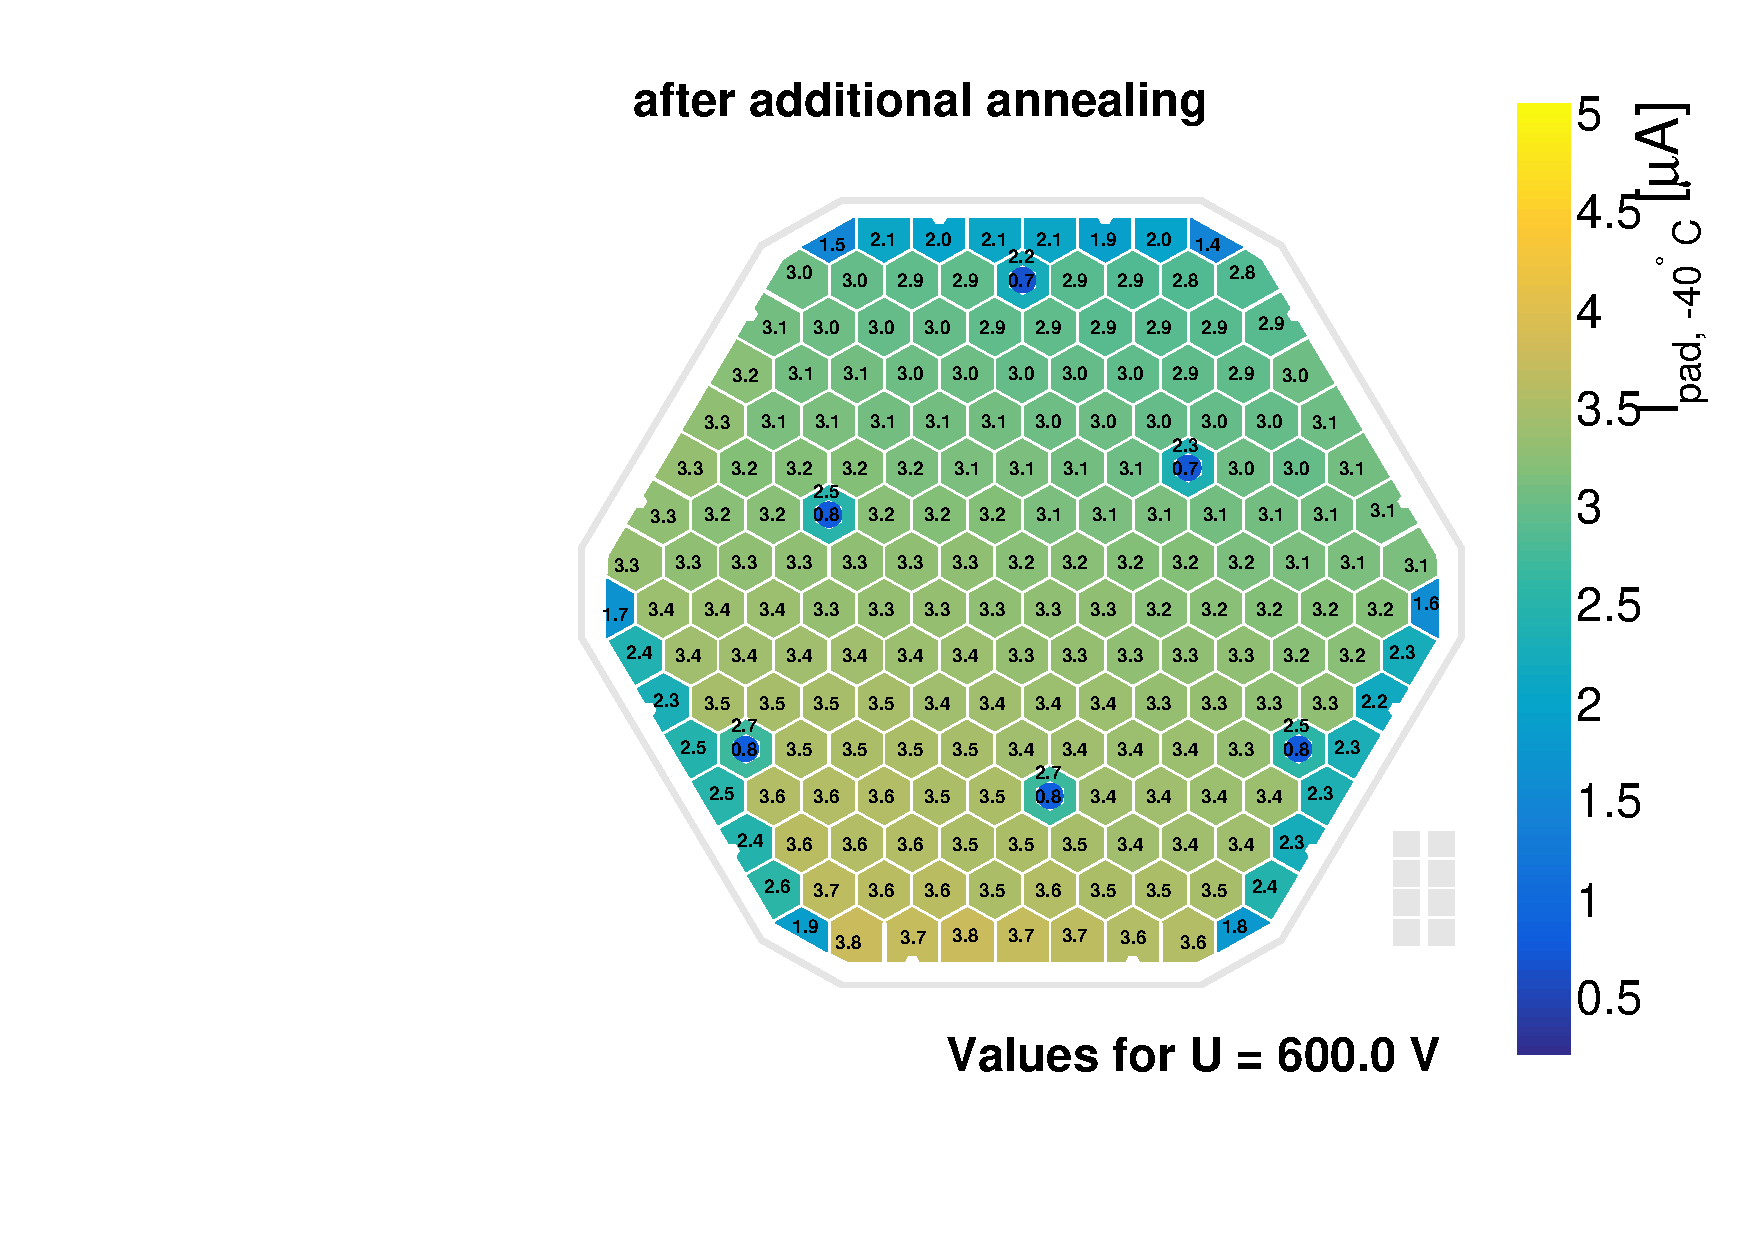
\includegraphics[width=0.7\textwidth]{plots/N4790_21.pdf}
      \caption{Round5, N4790\_21}
    \end{figure}

    \begin{figure}
      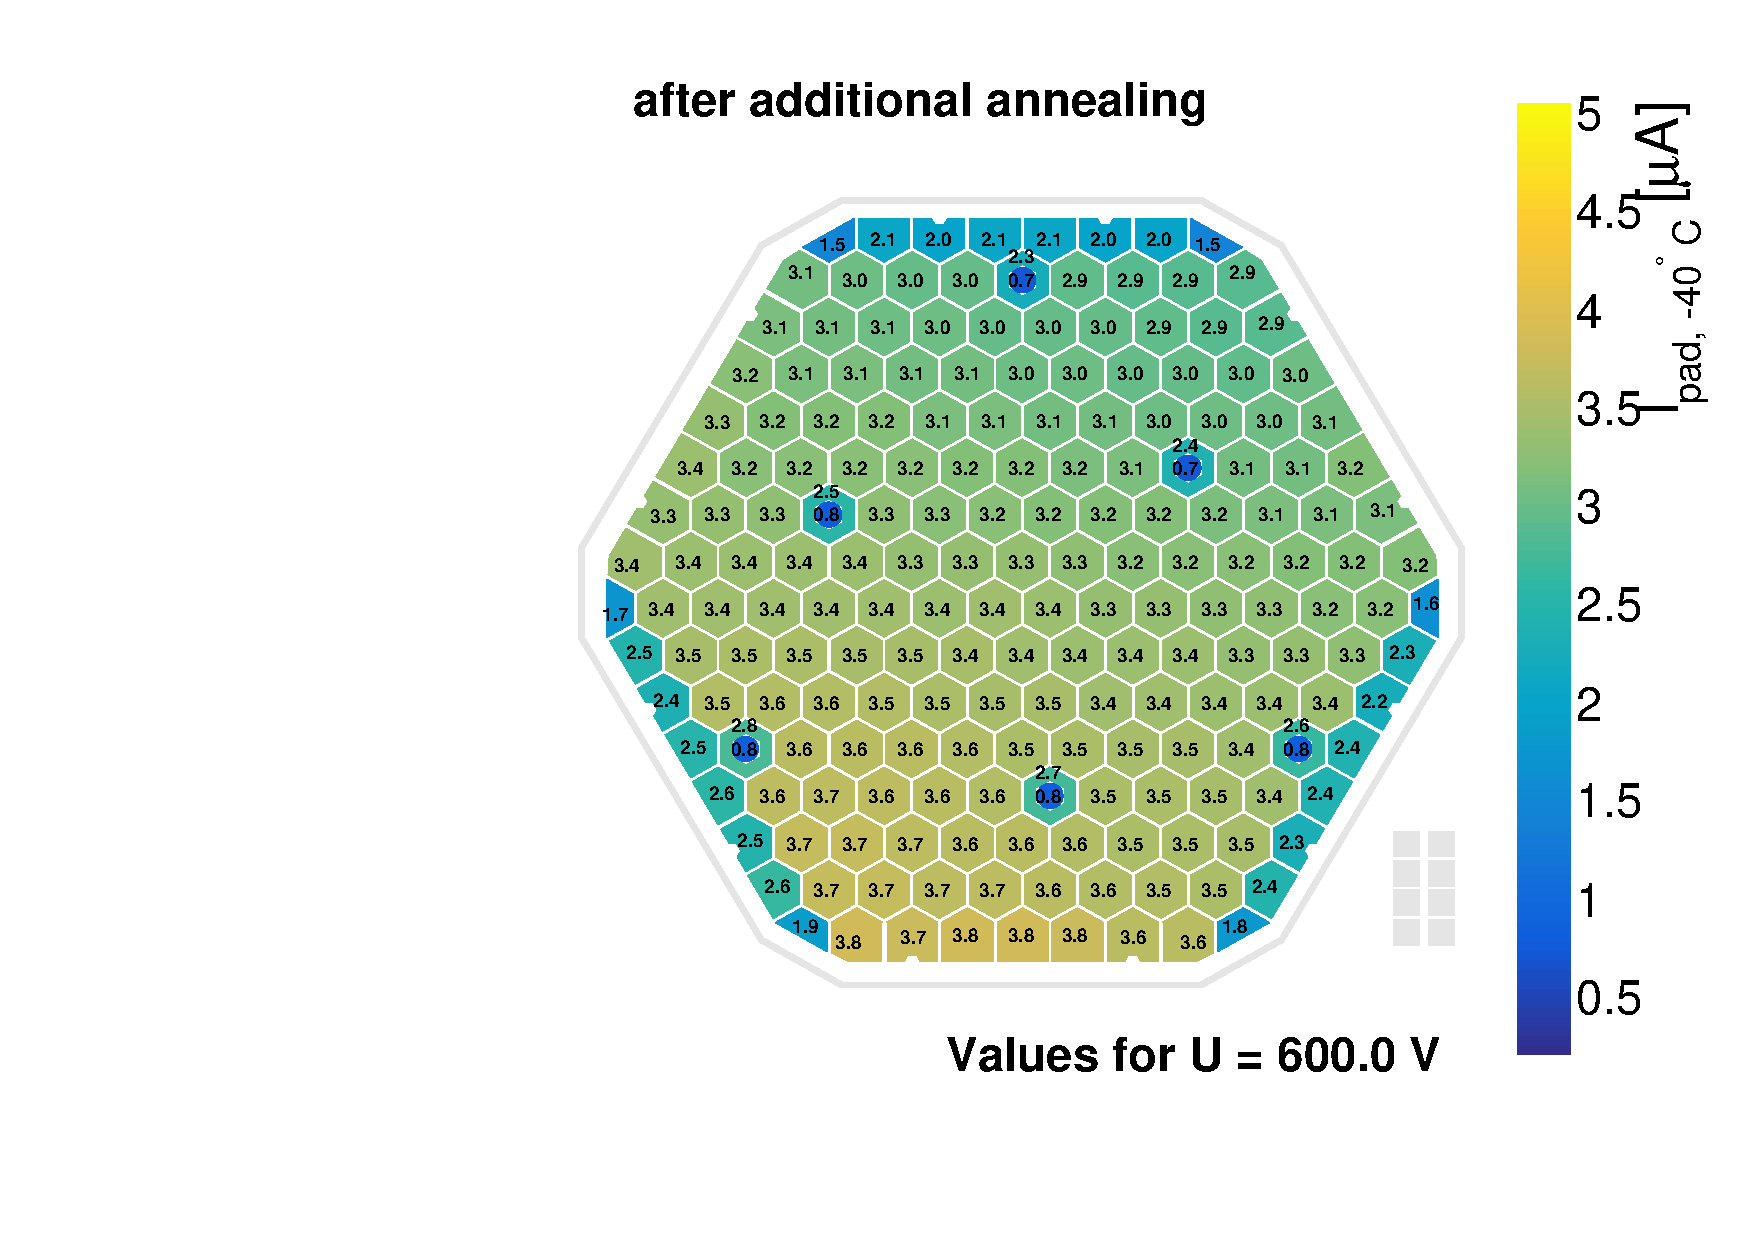
\includegraphics[width=0.7\textwidth]{plots/N4792_20.pdf}
      \caption{Round6, N4792\_20}
    \end{figure}

  \end{columns}
\end{frame}




\section{Annealing effect on CV Results}

\begin{frame}{CV results, N4790\_21}
  \begin{figure}
      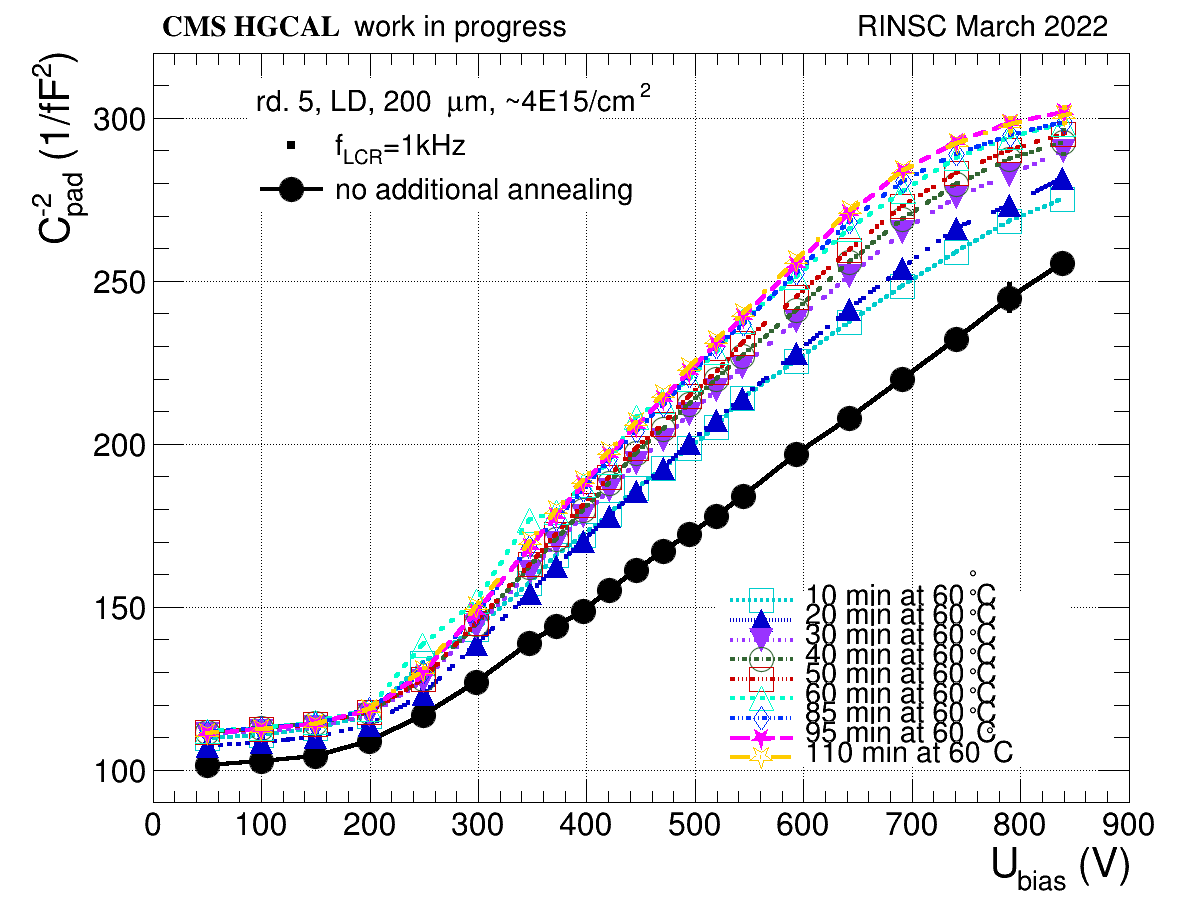
\includegraphics[width=.6\textwidth]{plots/annealing_CV_ch101_N4790_21.png}    
  \end{figure}
  \begin{itemize}
    % \item HexPlots as graphical representation of cell properties on the sensor
    \item We do see annealing effects
    \item Reached the limit of reversed annealing at around \alert{60 min}
    \item  Depletion voltage not reached 
  \end{itemize}
\end{frame}

\begin{frame}{CV results, N4790\_09}
  \begin{figure}
      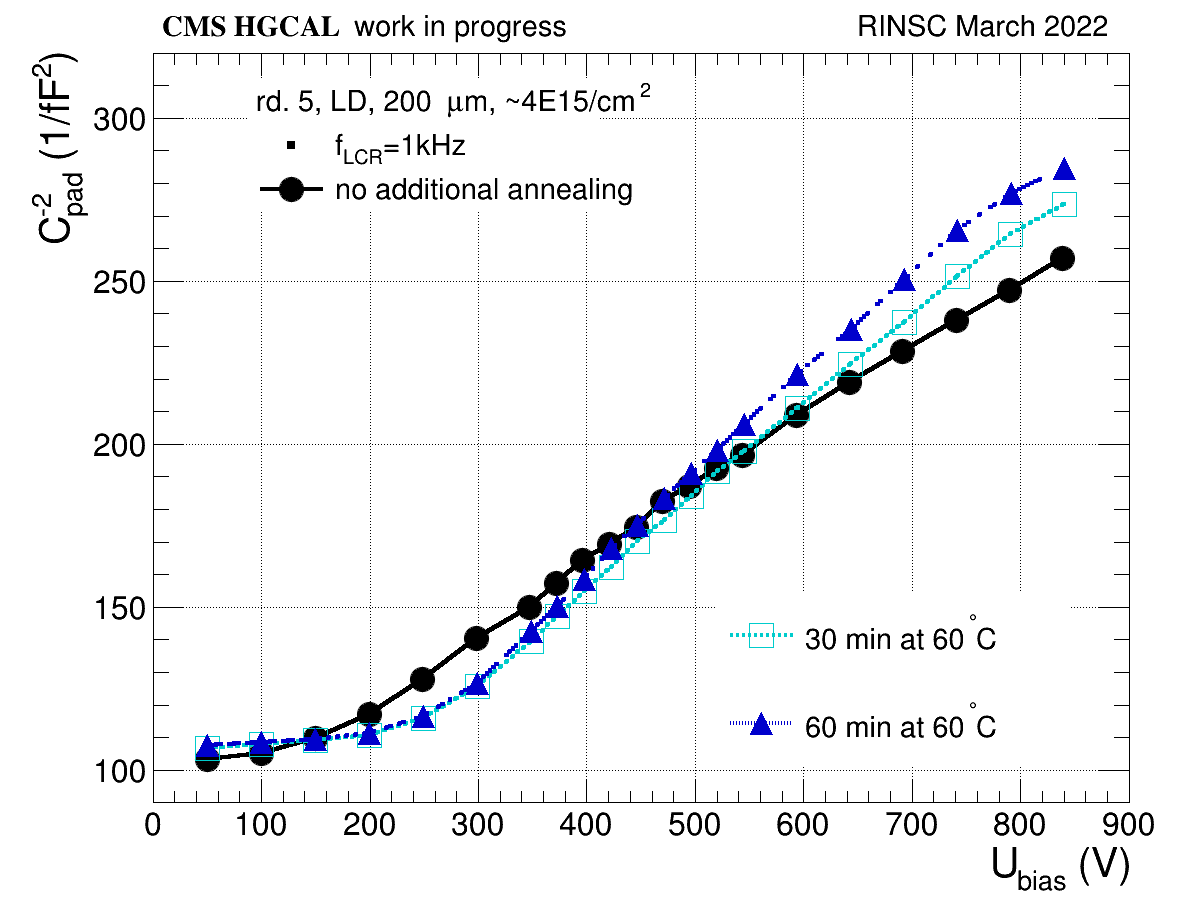
\includegraphics[width=.7\textwidth]{plots/annealing_CV_ch101_N4790_09.png}    
  \end{figure}
  \begin{itemize}
    \item CV curves
  \end{itemize}
\end{frame}

\begin{frame}{CV results, N4792\_07}
  \begin{figure}
      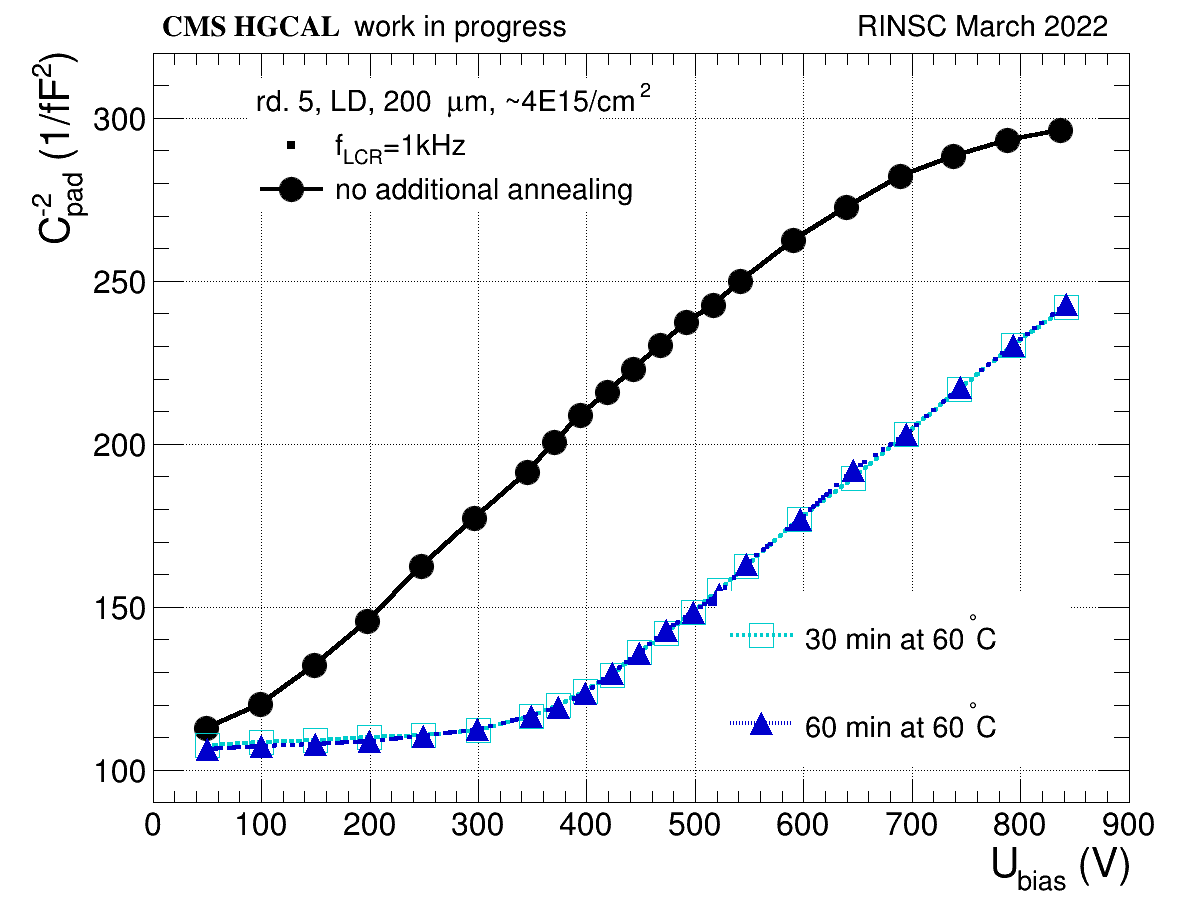
\includegraphics[width=.7\textwidth]{plots/annealing_CV_ch101_N4792_7.png}    
  \end{figure}
  \begin{itemize}
    \item CV curves
  \end{itemize}
\end{frame}






\section{Alpha plot}
\section{Leakage current vs. fluence behaviour}
\begin{frame}{Proto-A: example CV results}
  \begin{figure}
      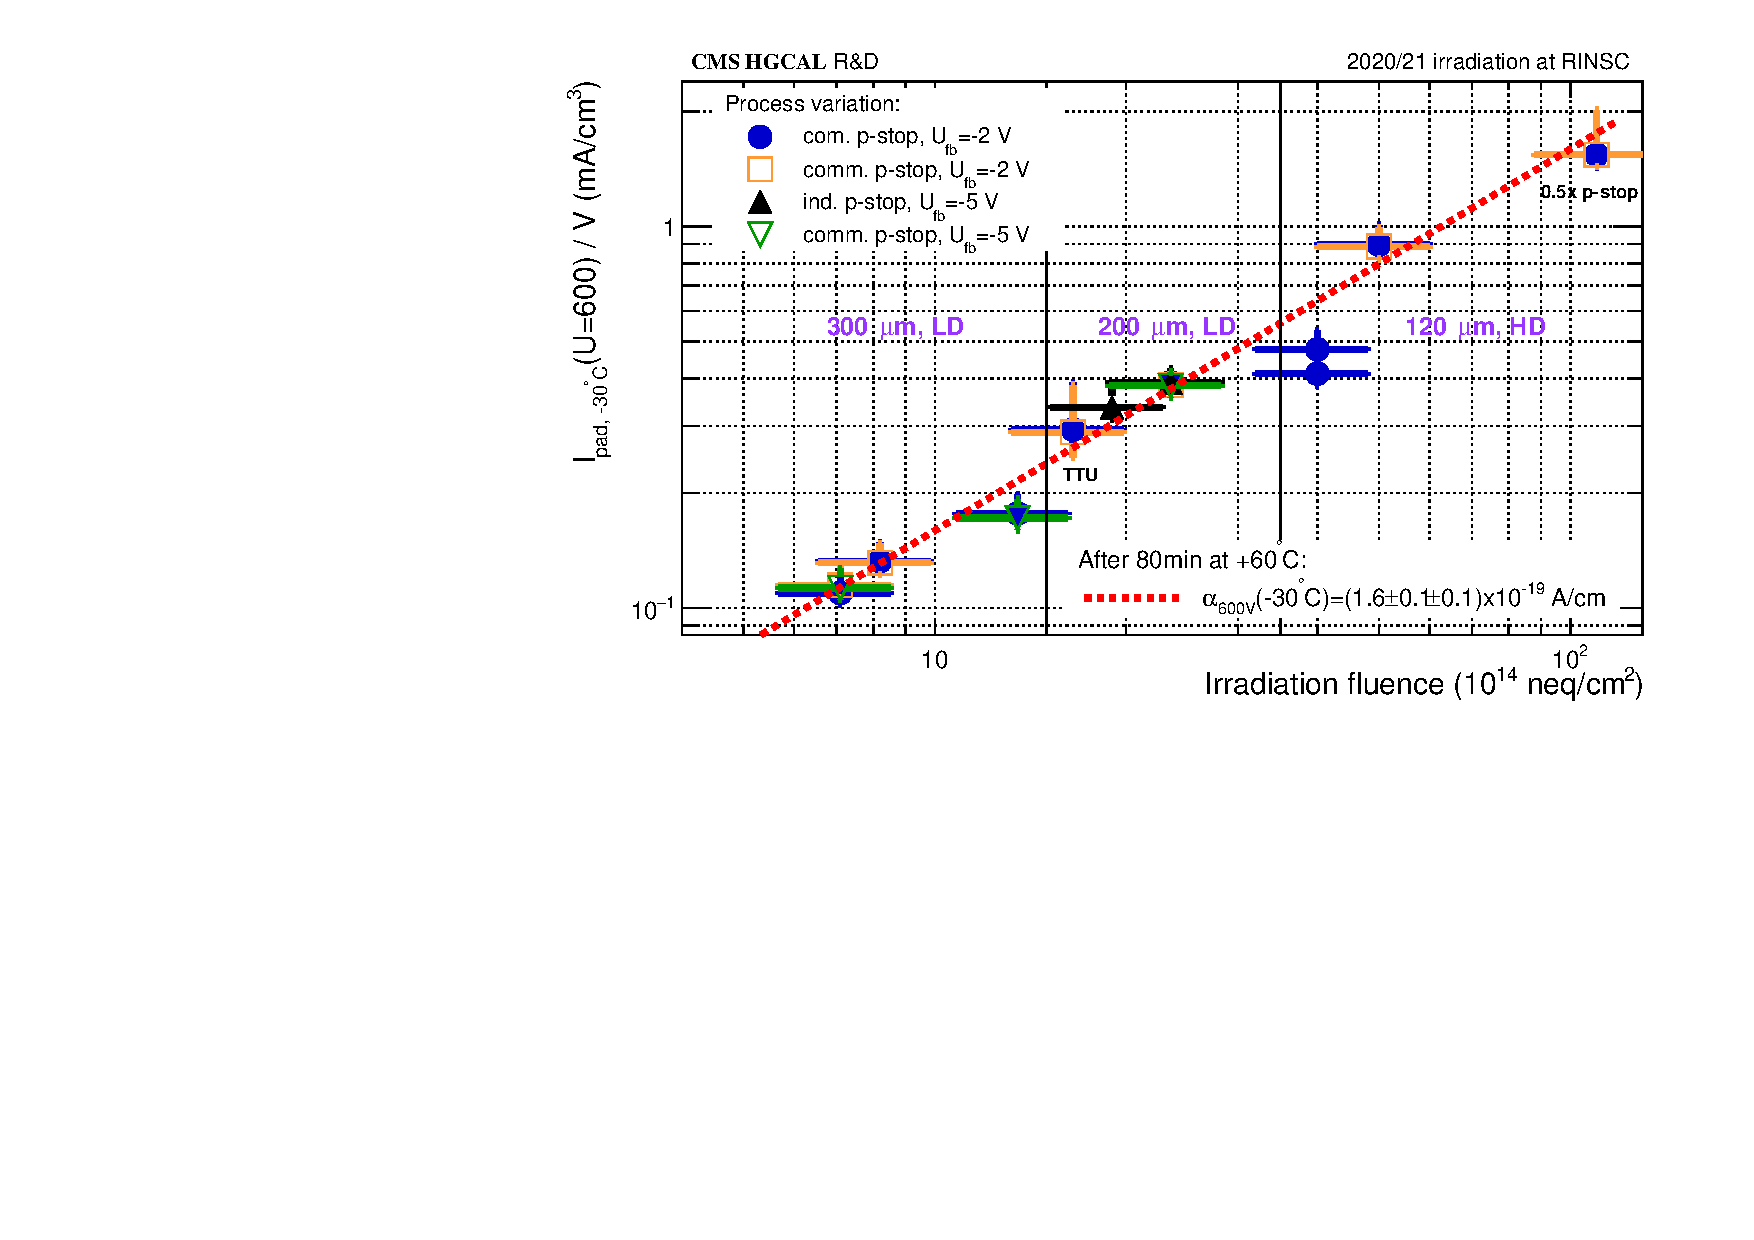
\includegraphics[width=0.6\textwidth]{plots/alpha_600V.pdf}    
  \end{figure}
  \begin{itemize}
    \item Round 5 and 6 sensors in general follow the current damage rate from previous campaigns
    \item Round 5 the sensor N4792\_7 seems to have received more annealing during the irradiation
    \item Round 6 has probably been annealed significantly more than 80 mins (values for the other sensors)
  \end{itemize}
\end{frame}


\section{Next steps}
\begin{frame}{Summary}
  \begin{itemize}
    % \scriptsize
    \item Clarify the irradiation setup with Nick to better understand the annealing during the irradiation
    \item Measure and analyze Round 7 \& 8 sensors
    % \item Test throughput 20 sensors per week
    % \item Shortage of LCR meters problem resolved
  \end{itemize}
\end{frame}

\appendix

\begin{frame}{Backup}
	\center
	\huge
	Backup slides
\end{frame}




\begin{frame}{RINSC irradiation, Round 5}
    \begin{figure}
        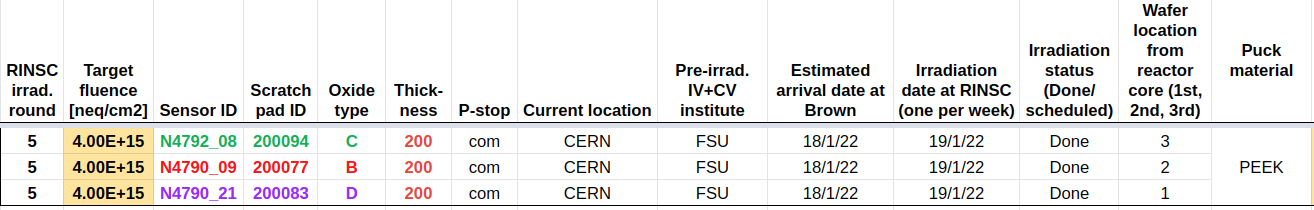
\includegraphics[width=.7\textwidth]{plots/Round_5_sensors.png}
        \caption{Round 5, sensors, N4792\_7 instead of N4792\_8}
    \end{figure}
    \begin{figure}
      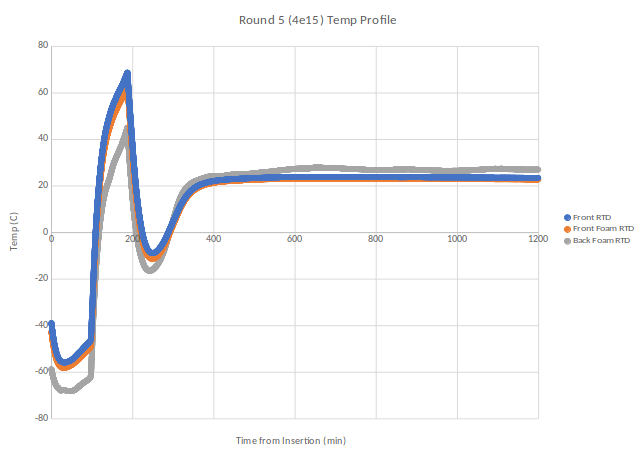
\includegraphics[width=.5\textwidth]{plots/Round5_temp_profile.png}
      \caption{Round 5, temperature profile}
    \end{figure}
\end{frame}

\begin{frame}{RINSC irradiation, Round 6}
    \begin{figure}
        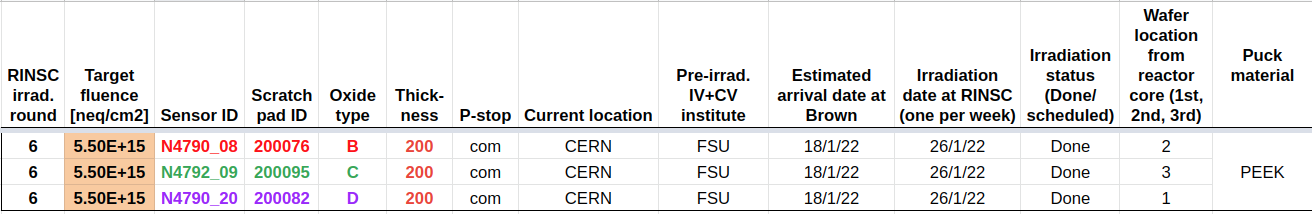
\includegraphics[width=.7\textwidth]{plots/Round_6_sensors.png}
        \caption{Round 6, sensors}
    \end{figure}
    \begin{figure}
      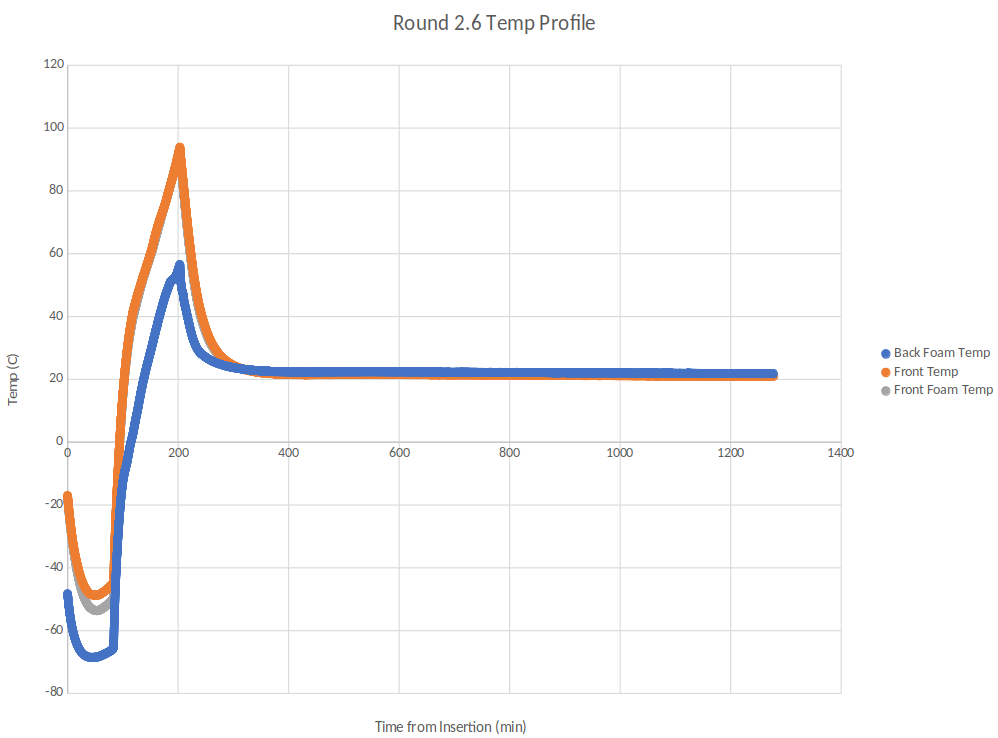
\includegraphics[width=.5\textwidth]{plots/Round6_temp_profile.png}
      \caption{Round 6, temperature profile}
    \end{figure}
\end{frame}


\end{document}


